\documentclass{article}
\usepackage[utf8]{inputenc}
\usepackage{graphicx}
\usepackage{parskip}
\title{StateCharts}
\author{Umang Deshpande and Akshay Hegde}
\date{June 2017}

\begin{document}
\maketitle

\section{Objectives:}
\begin{itemize}
    \item Understanding the basics of Statecharts
    \item Implementing a Timer Bomb game
\end{itemize}
\section{Prerequisite:}
\begin{itemize}
    \item Statemachine implementation
    \item Please go through the resource section to understand how to implement a statechart
\end{itemize}
\section{Problem Statement:}
The time bomb has a control panel with an GLCD that shows the current value of the timeout and three buttons: UP, DOWN, and ARM. The user begins with setting up the time bomb using the UP and DOWN buttons to adjust the timeout in one-second steps. Once the desired timeout is selected, the user can arm the bomb by pressing the ARM button. When armed, the bomb starts decrementing the timeout every second and explodes when the timeout reaches zero. An additional safety feature is the option to defuse an armed bomb by entering a secret code. The secret defuse code is a certain combination of the UP,DOWN and LEFT buttons. Of course, the defuse code must be correctly entered before the bomb times out.\\
In this lab you have to design a \textbf{Timer Bomb} using 4 switches present on the game console. Timer Bomb has 4 modes of operation. \textit{Idle, setTimer, autoTimer, bombExplode} and \textit{ bombDiffused}.
\section{Idle Mode:}
\begin{itemize}
    \item Initially controller will be in Idle state.
    \item Display some animation on start as shown in Fig1 and Fig2.
    \item After animation, display text ENTER as shown in Fig3 and wait till LEFT key press.
\end{itemize}
\begin{center}
   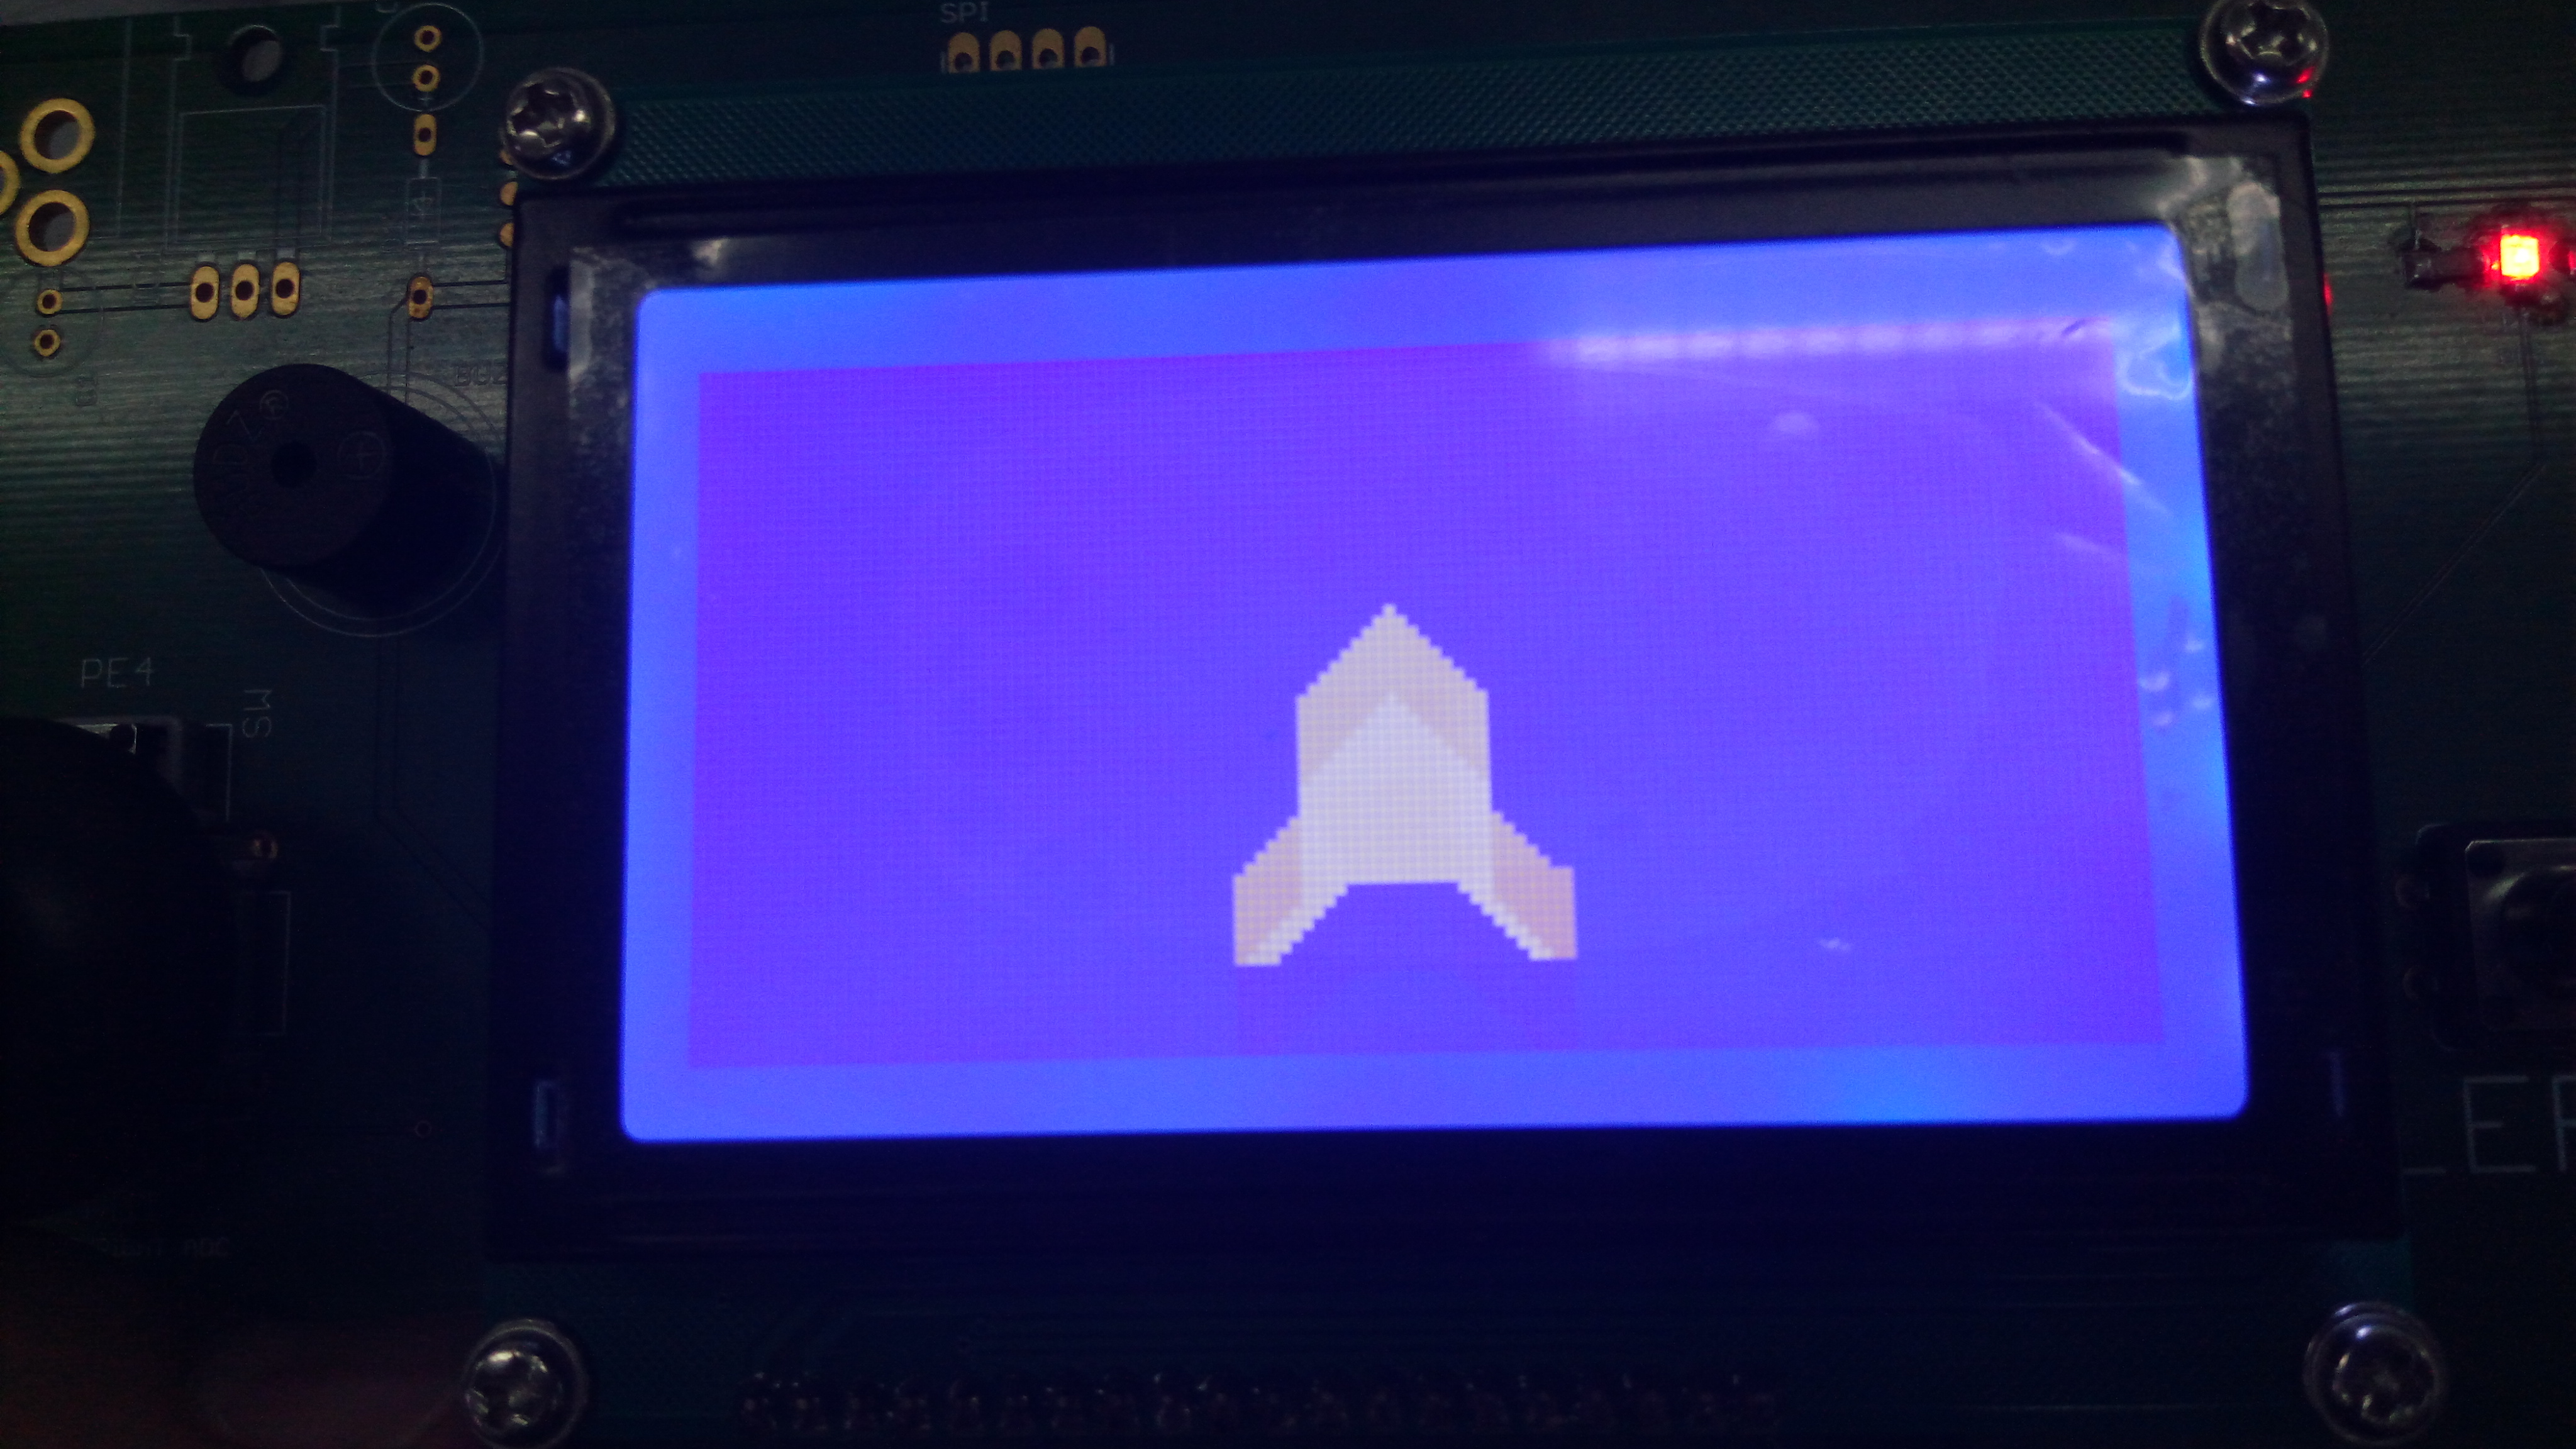
\includegraphics[width=8cm]{rocket1}
   \\Fig1: Rocket1
   \\[2\baselineskip]
   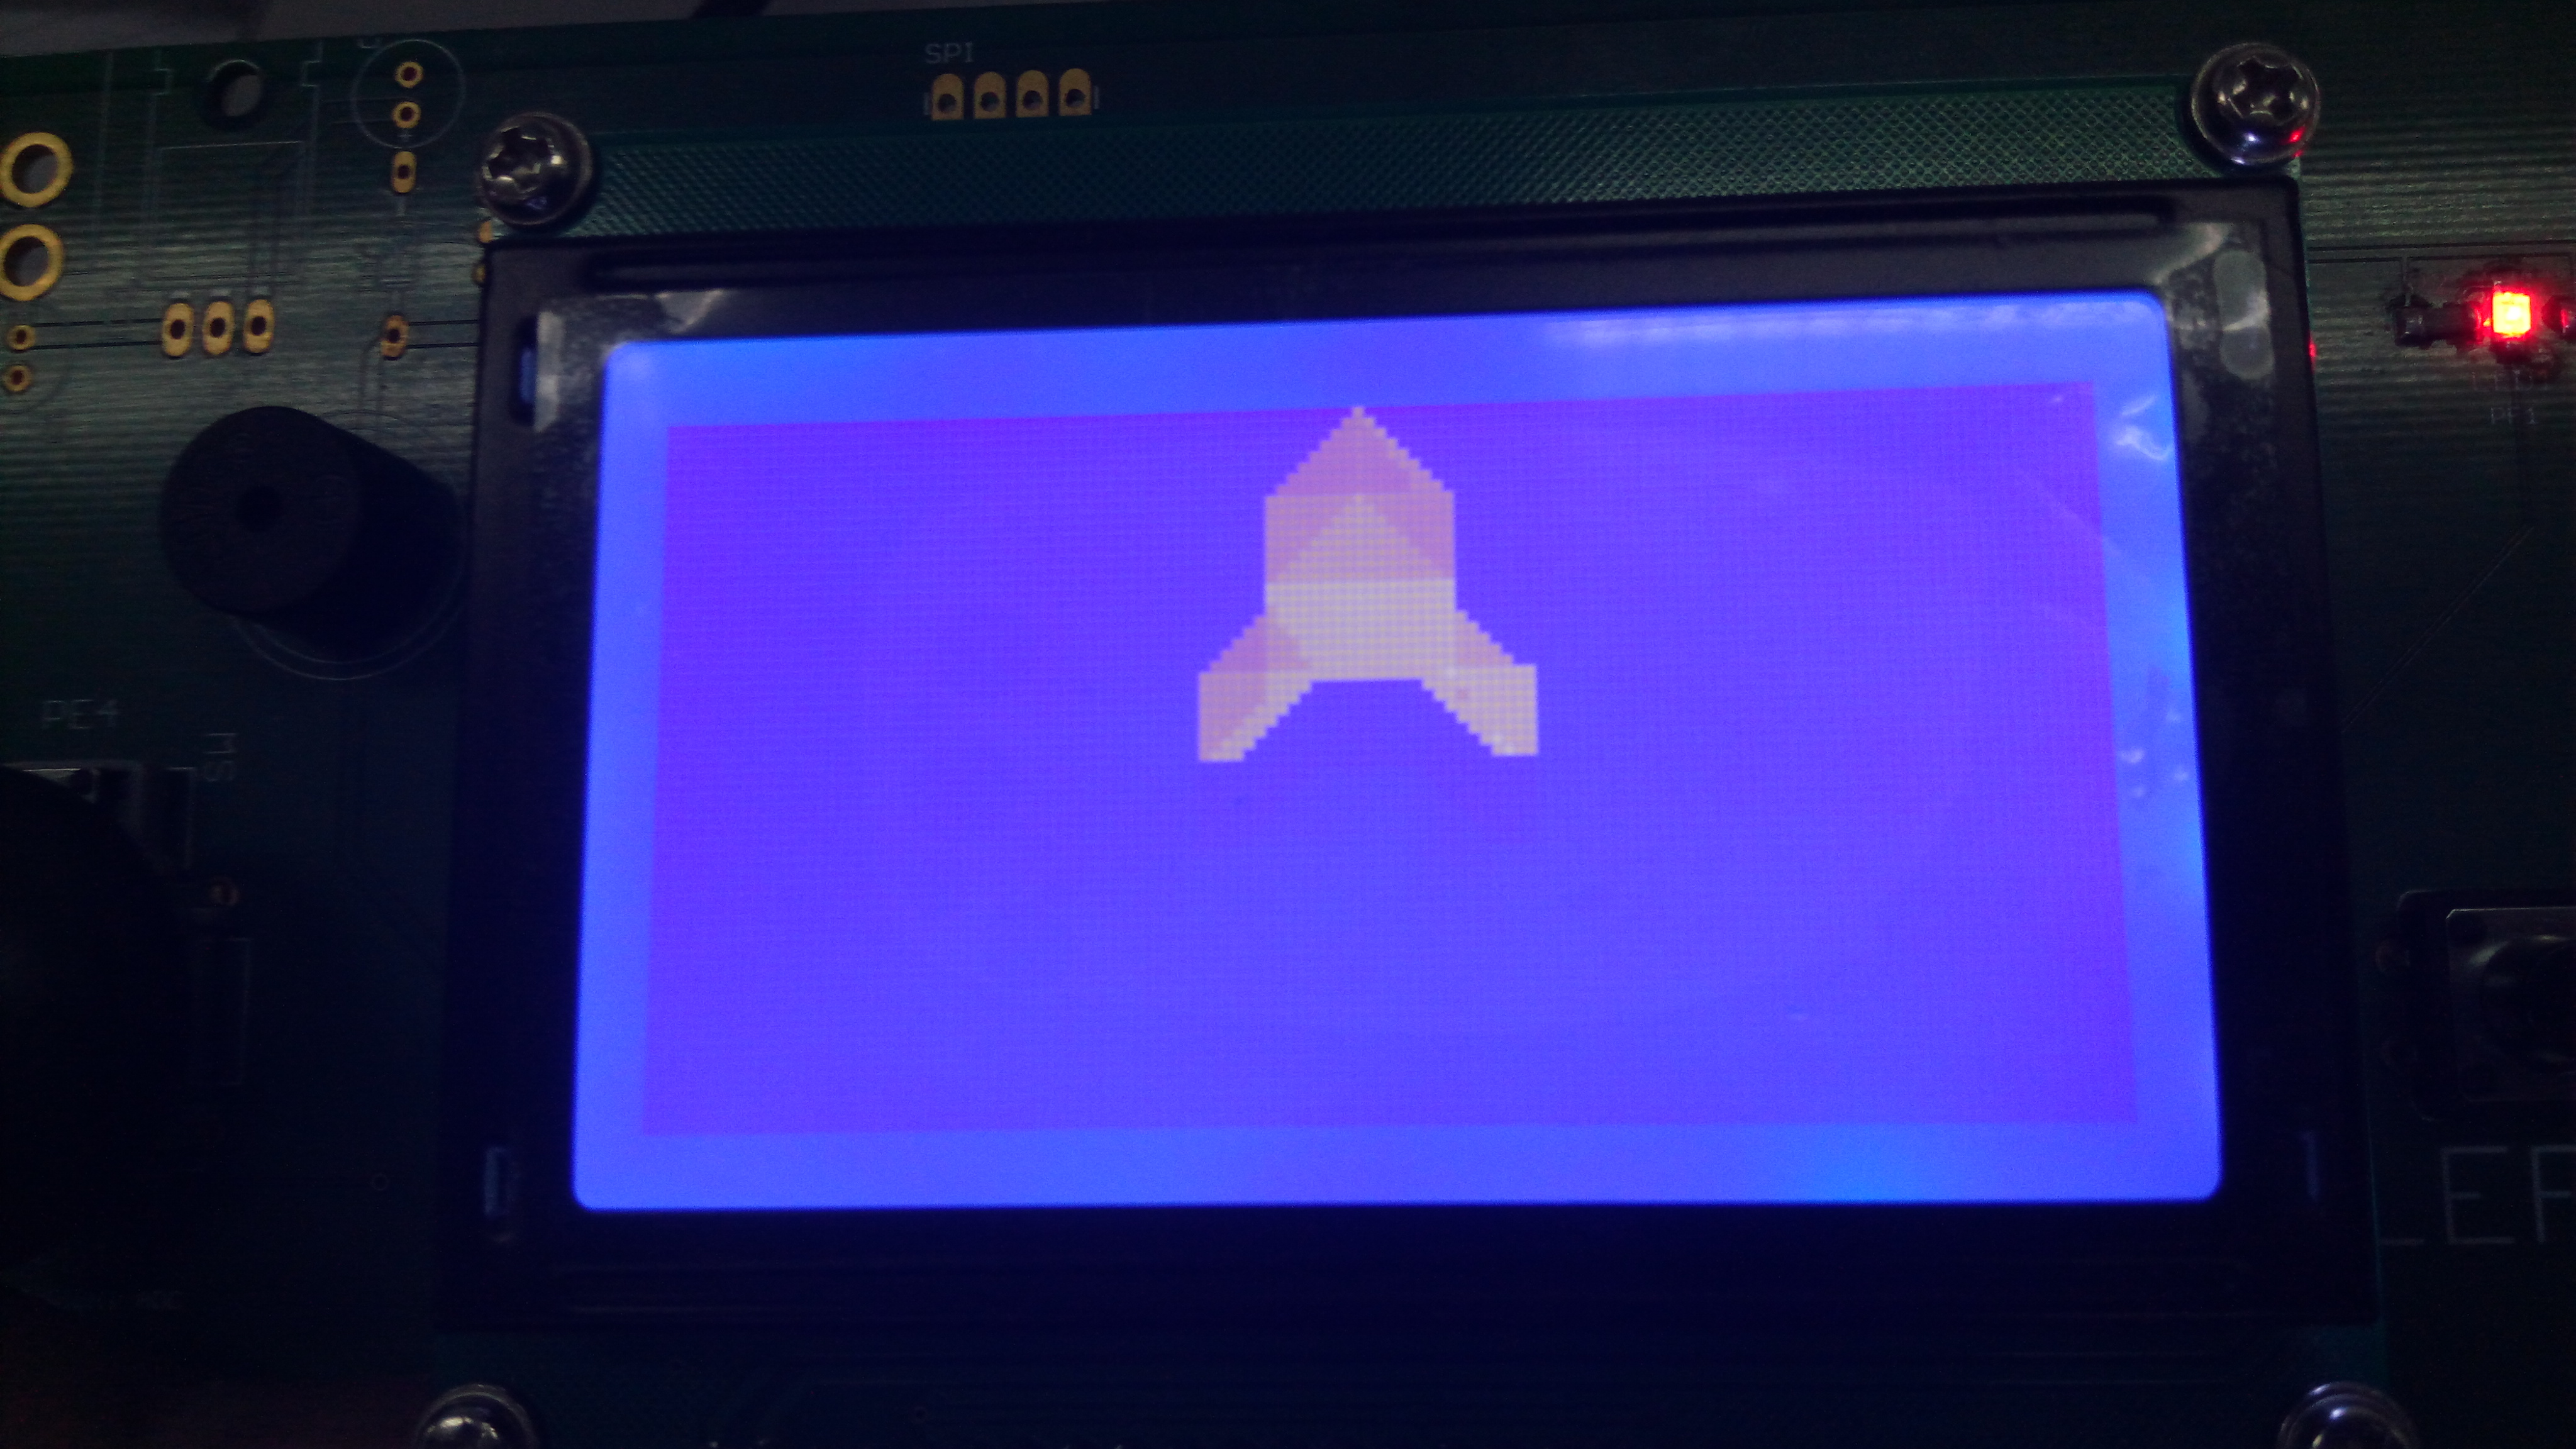
\includegraphics[width=8cm]{rocket2}
   \\Fig2: Rocket2
   \\[2\baselineskip]

   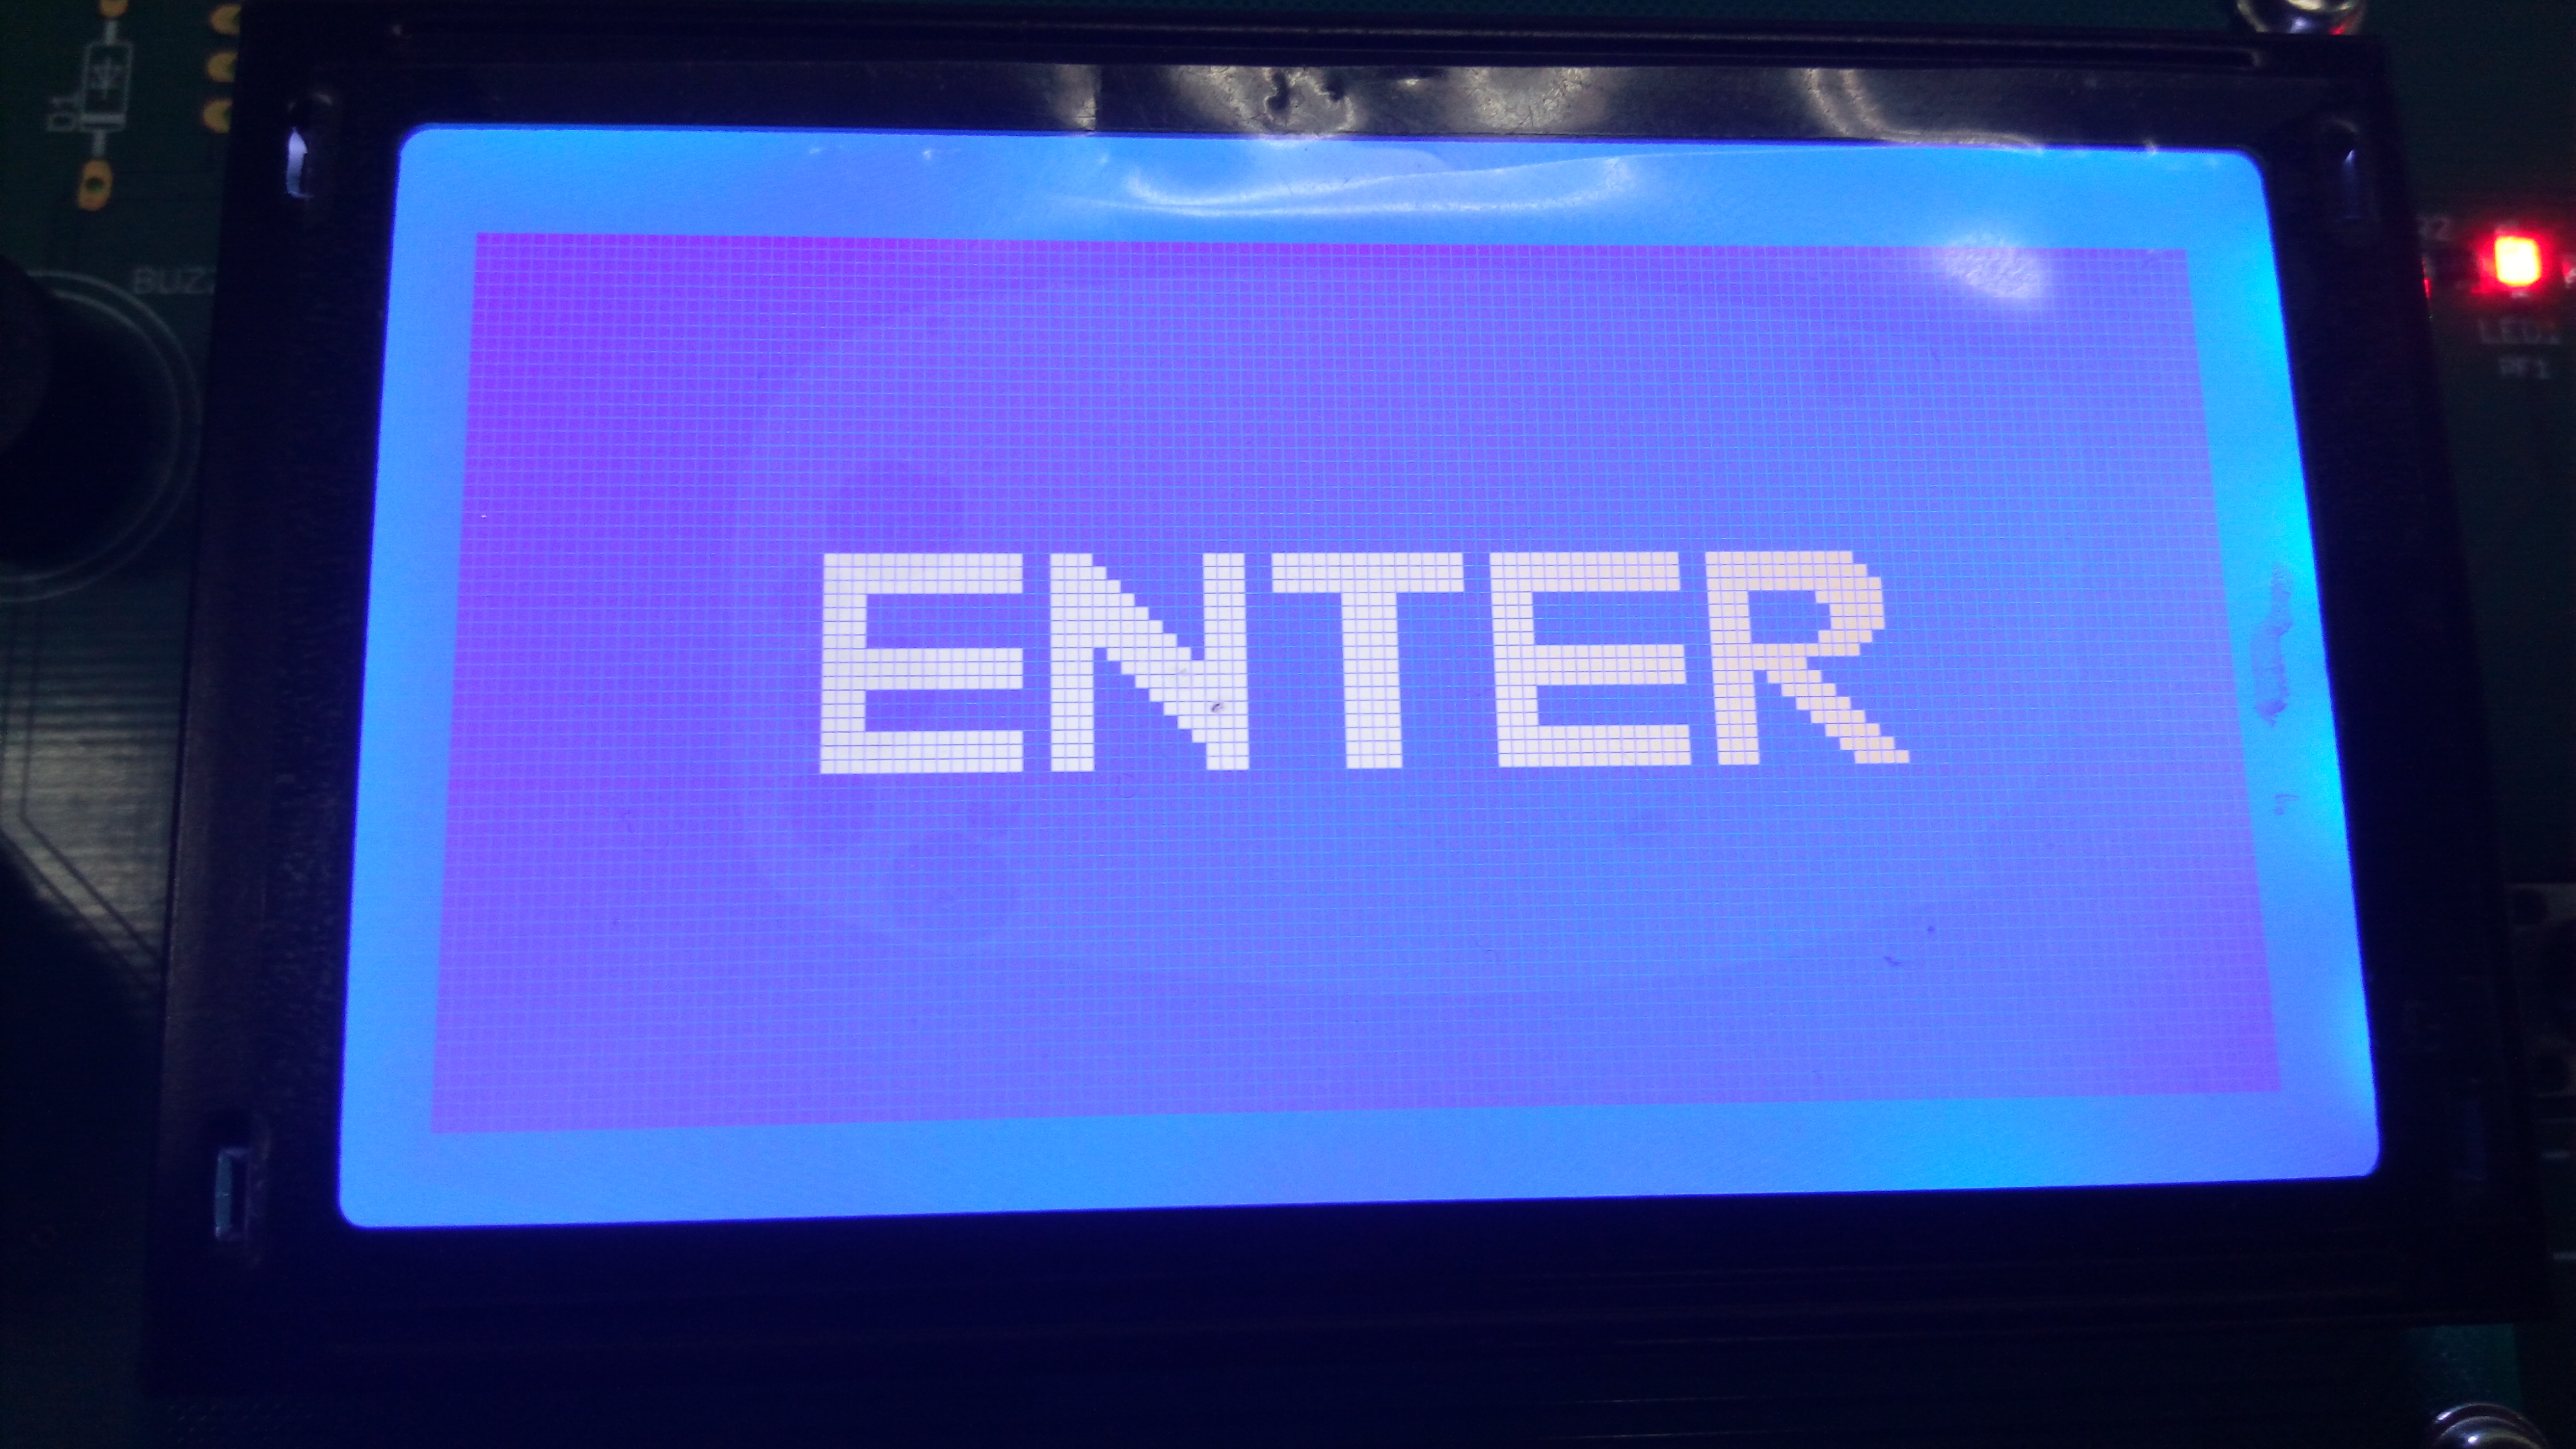
\includegraphics[width=8cm]{Enter.png}
   \\Fig3: Enter
   \\[2\baselineskip]

 \end{center}

\section{SetTimer Mode:}
\begin{itemize}
    \item Once LEFT key is pressed the controller will then enter in setTimer mode.
    \item In setTimer mode a 4 digit timer should be displayed as shown in Fig4. 
    \item Timer range is from 2 minutes to 10 seconds.
    \item UP and DOWN switches are used to increment and decrement the timer as shown in Fig5.
    \item RIGHT switch is used to arm the bomb.
    \item Instructions for the same should be displayed on screen describing the function of each switch.Wait till the right switch is pressed.
\end{itemize}
\begin{center}
   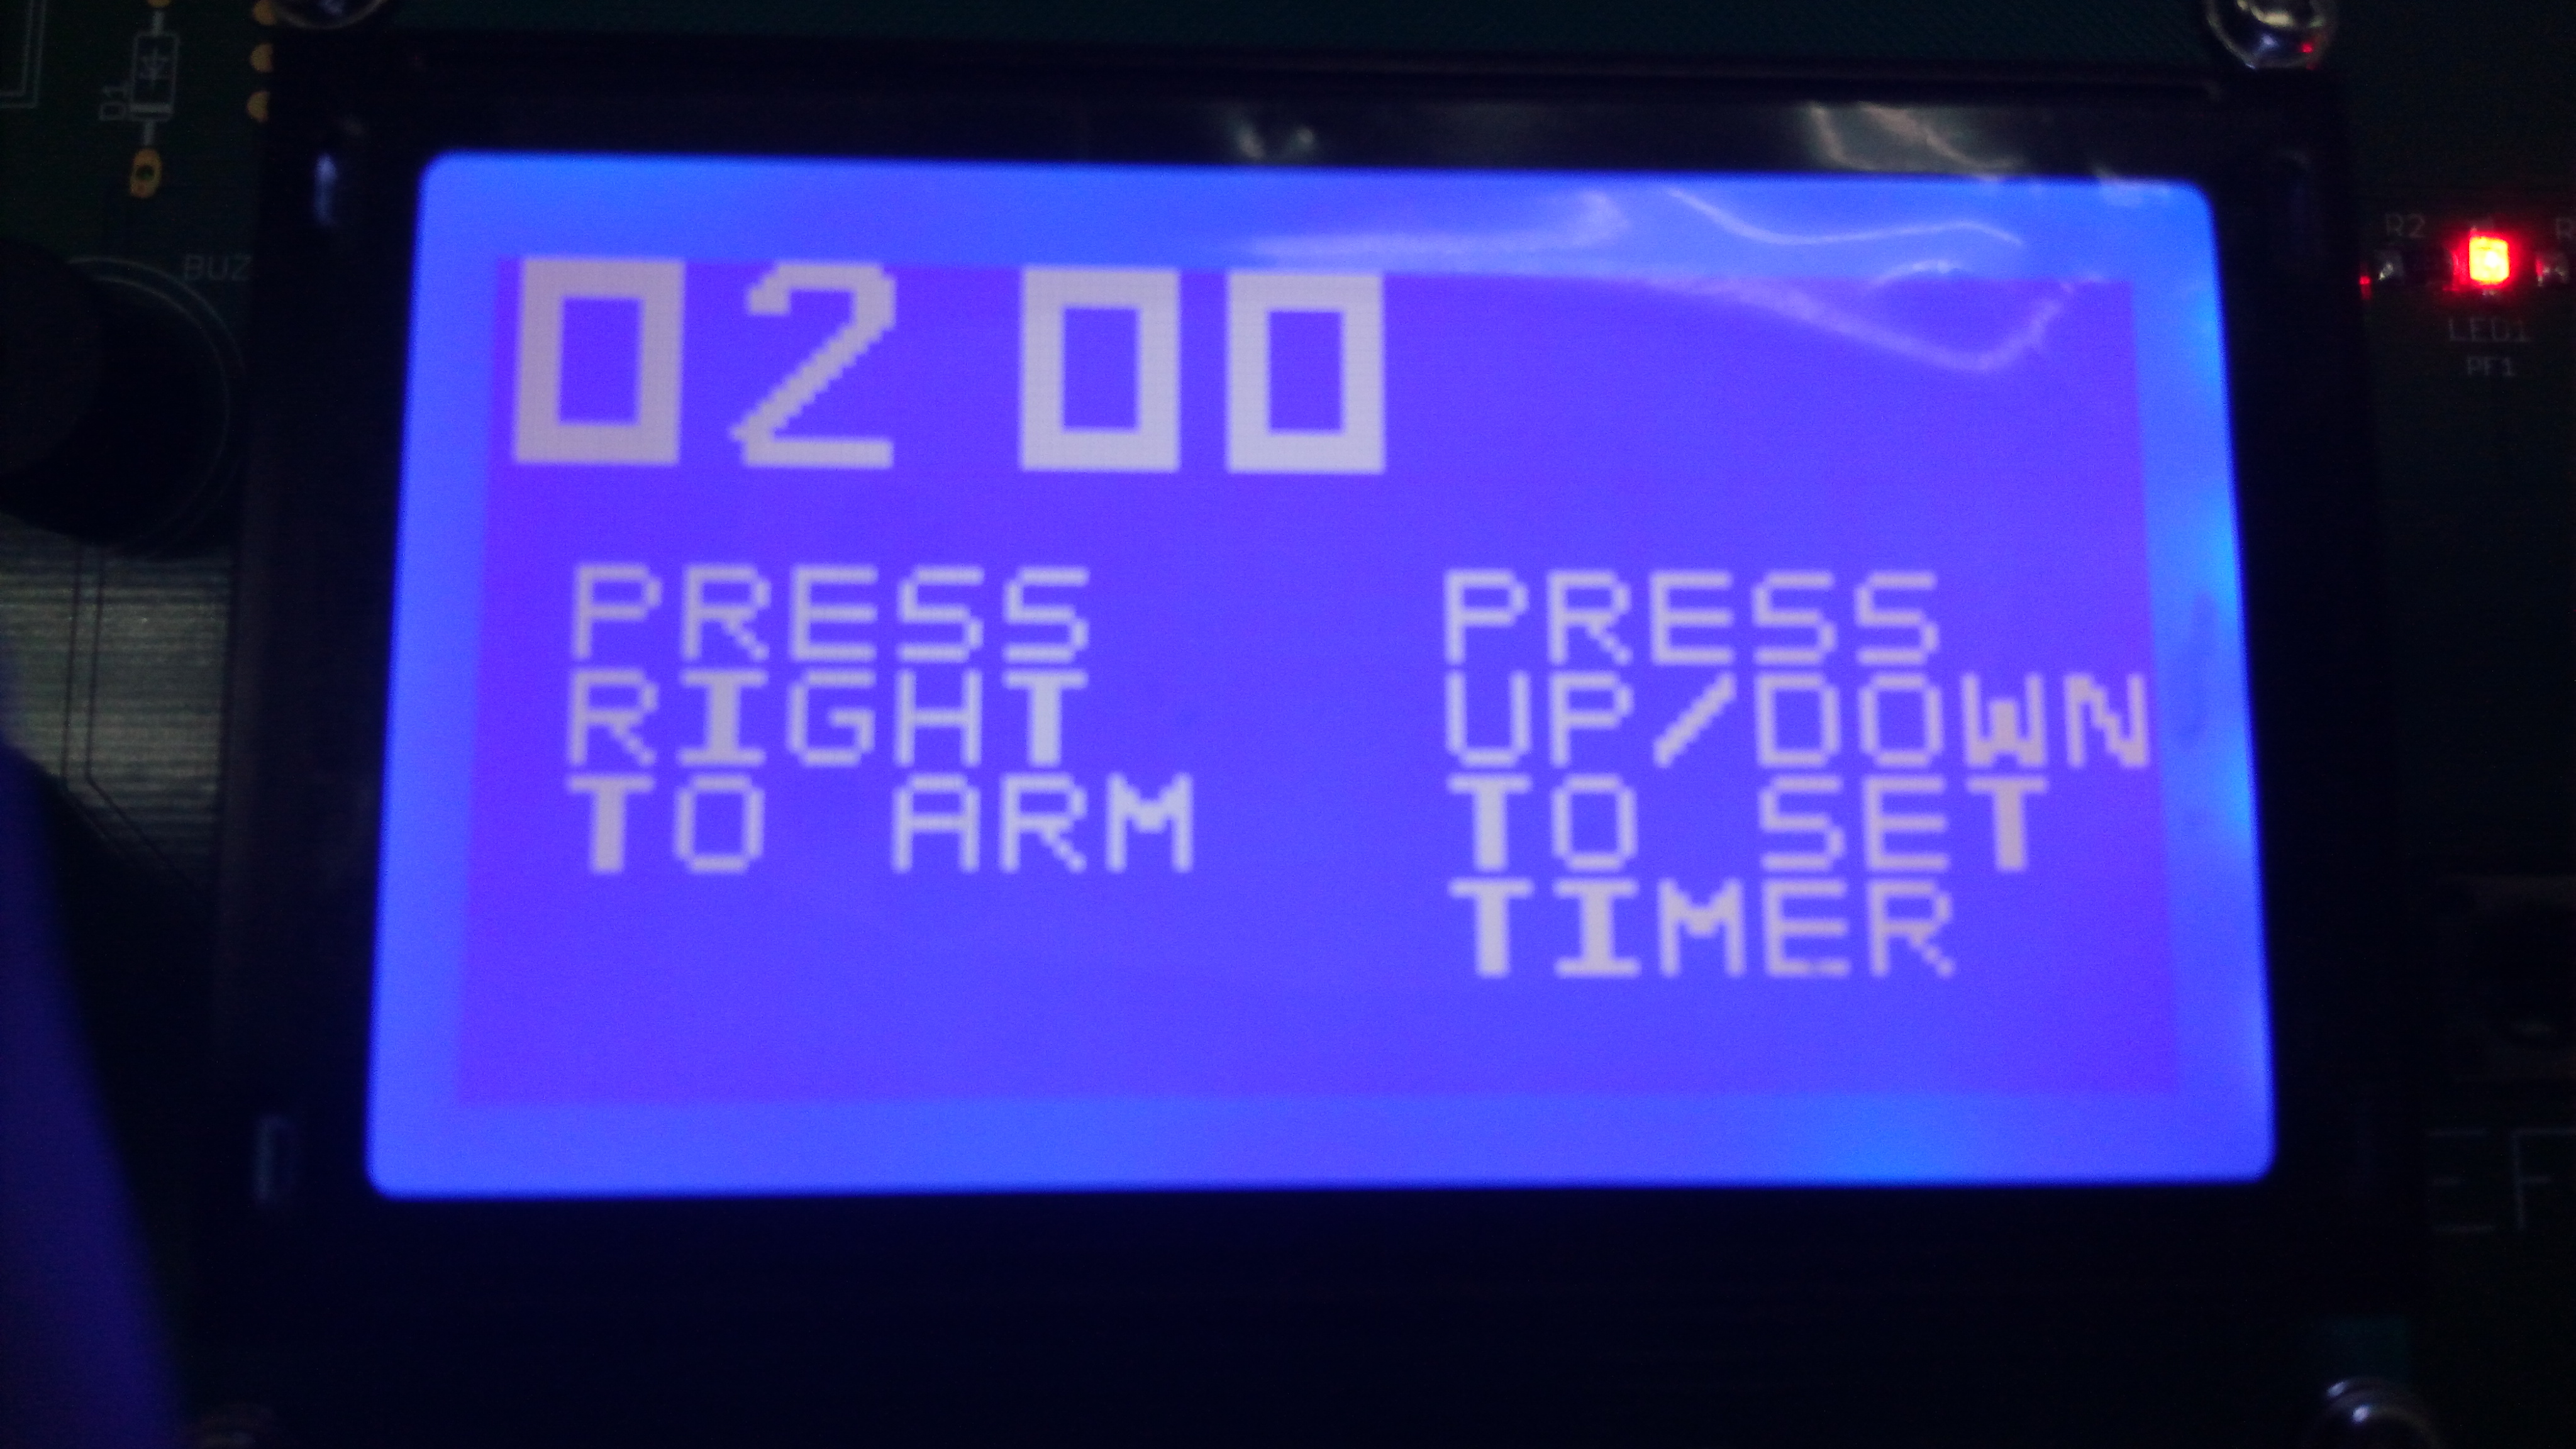
\includegraphics[width=8cm]{setTimer1}
   \\Fig4: setTimer1
   \\[2\baselineskip]
   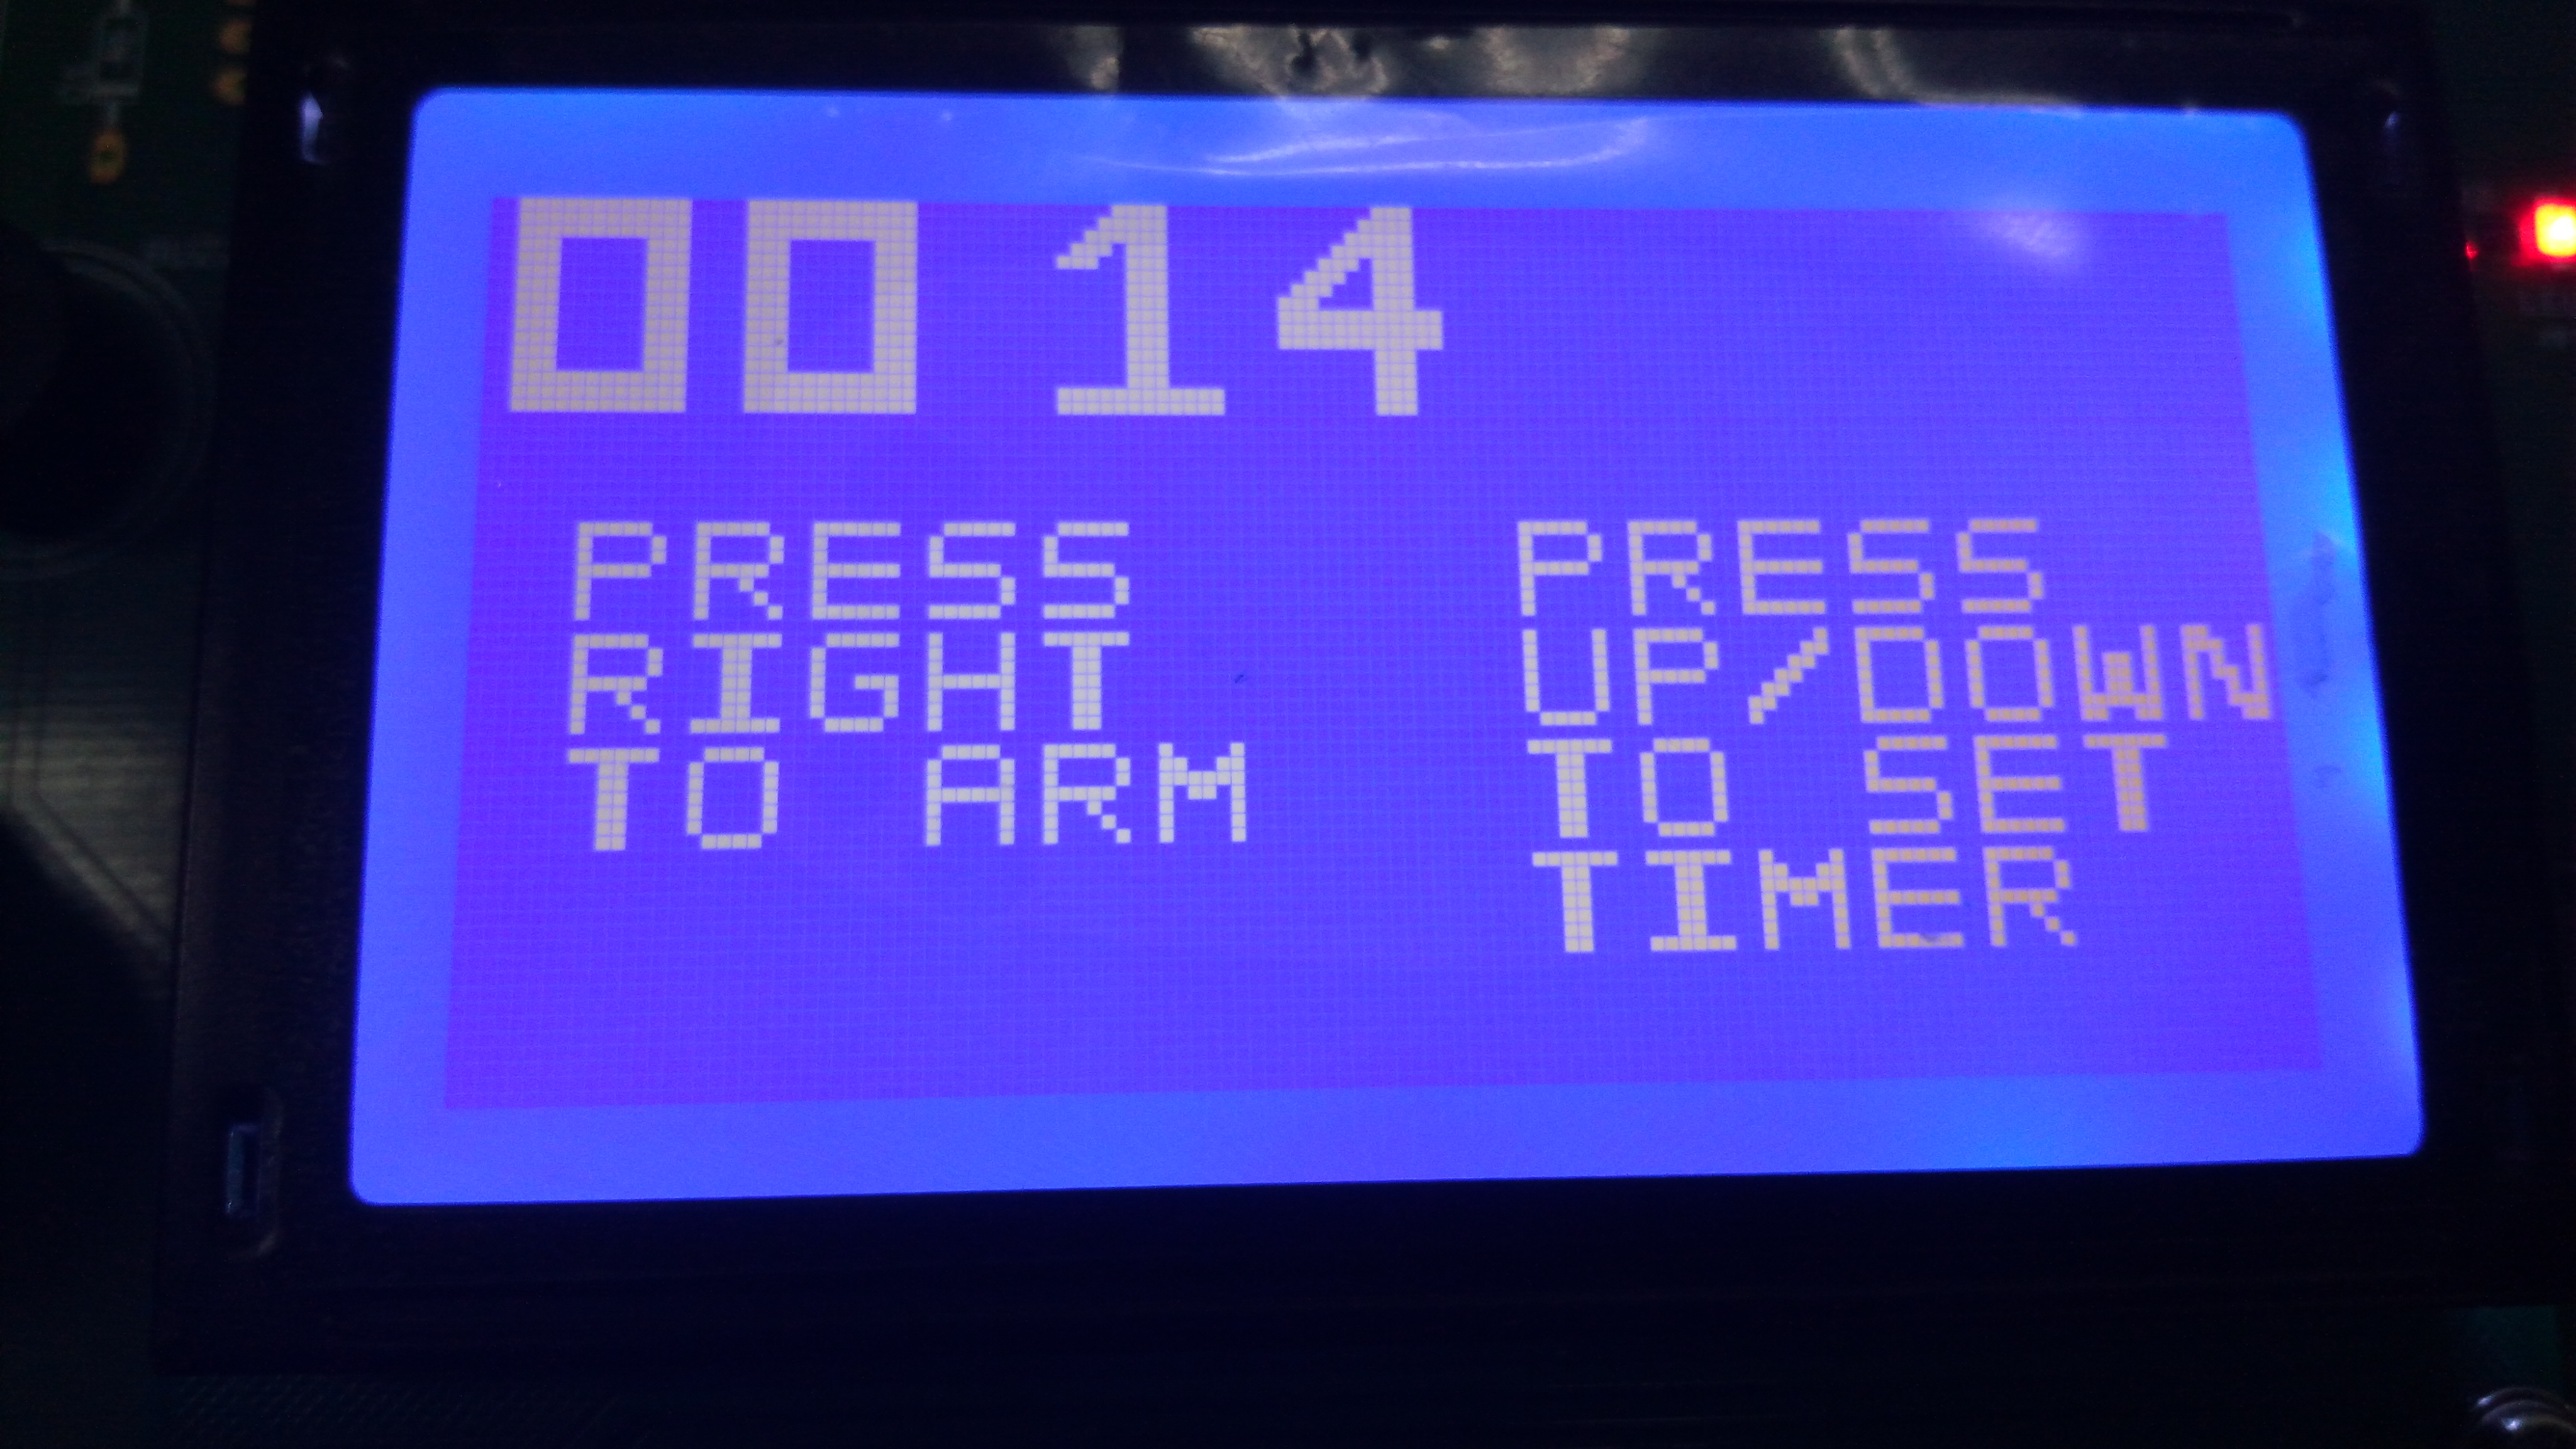
\includegraphics[width=8cm]{setTimer2}
   \\Fig5: setTimer2
   \\[2\baselineskip]
 \end{center}
\section{autoTimer Mode:}
\begin{itemize}
    \item Once RIGHT switch is pressed the controller will then enter in autoTimer mode.
    \item In autoTimer mode the timer should decrement automatically after every second as shown in Fig6 and Fig7. 
    \item Timer starts from the set time till value reaches zero
    \item A bomb should be displayed along with the timer display.
\end{itemize}
\begin{center}
   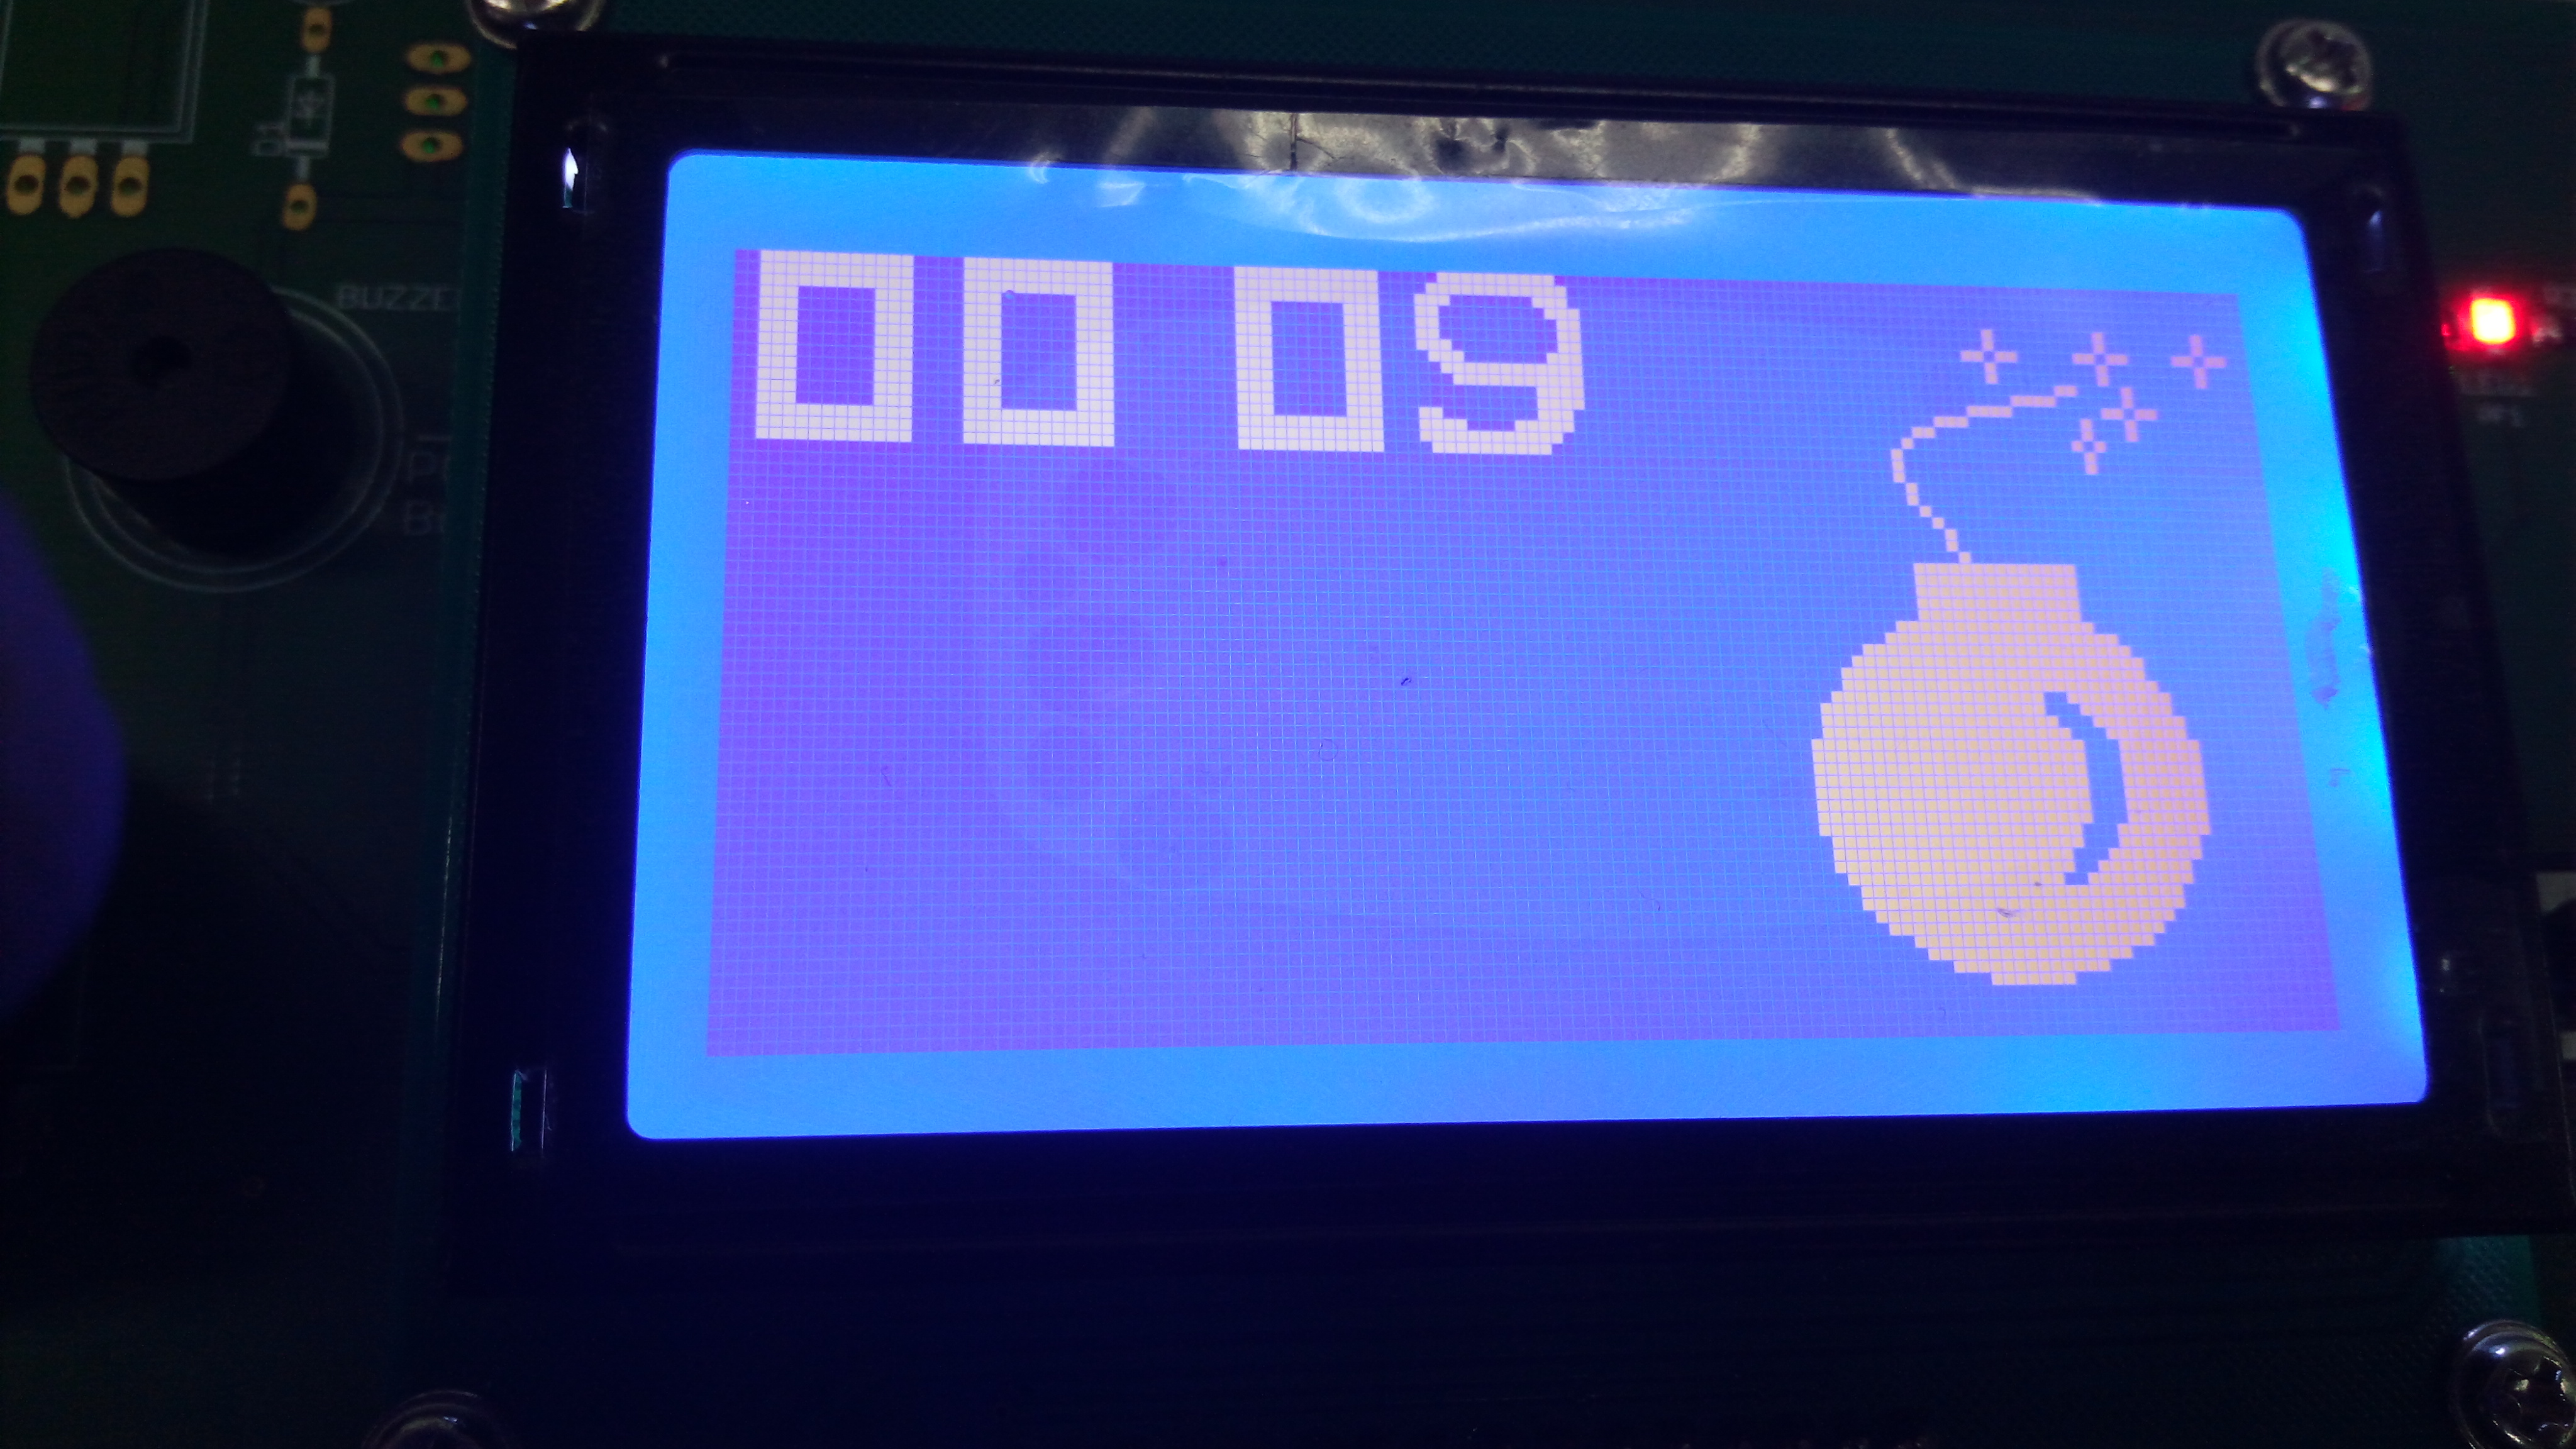
\includegraphics[width=8cm]{autoTimer1}
   \\Fig6: setTimer1
   \\[2\baselineskip]
   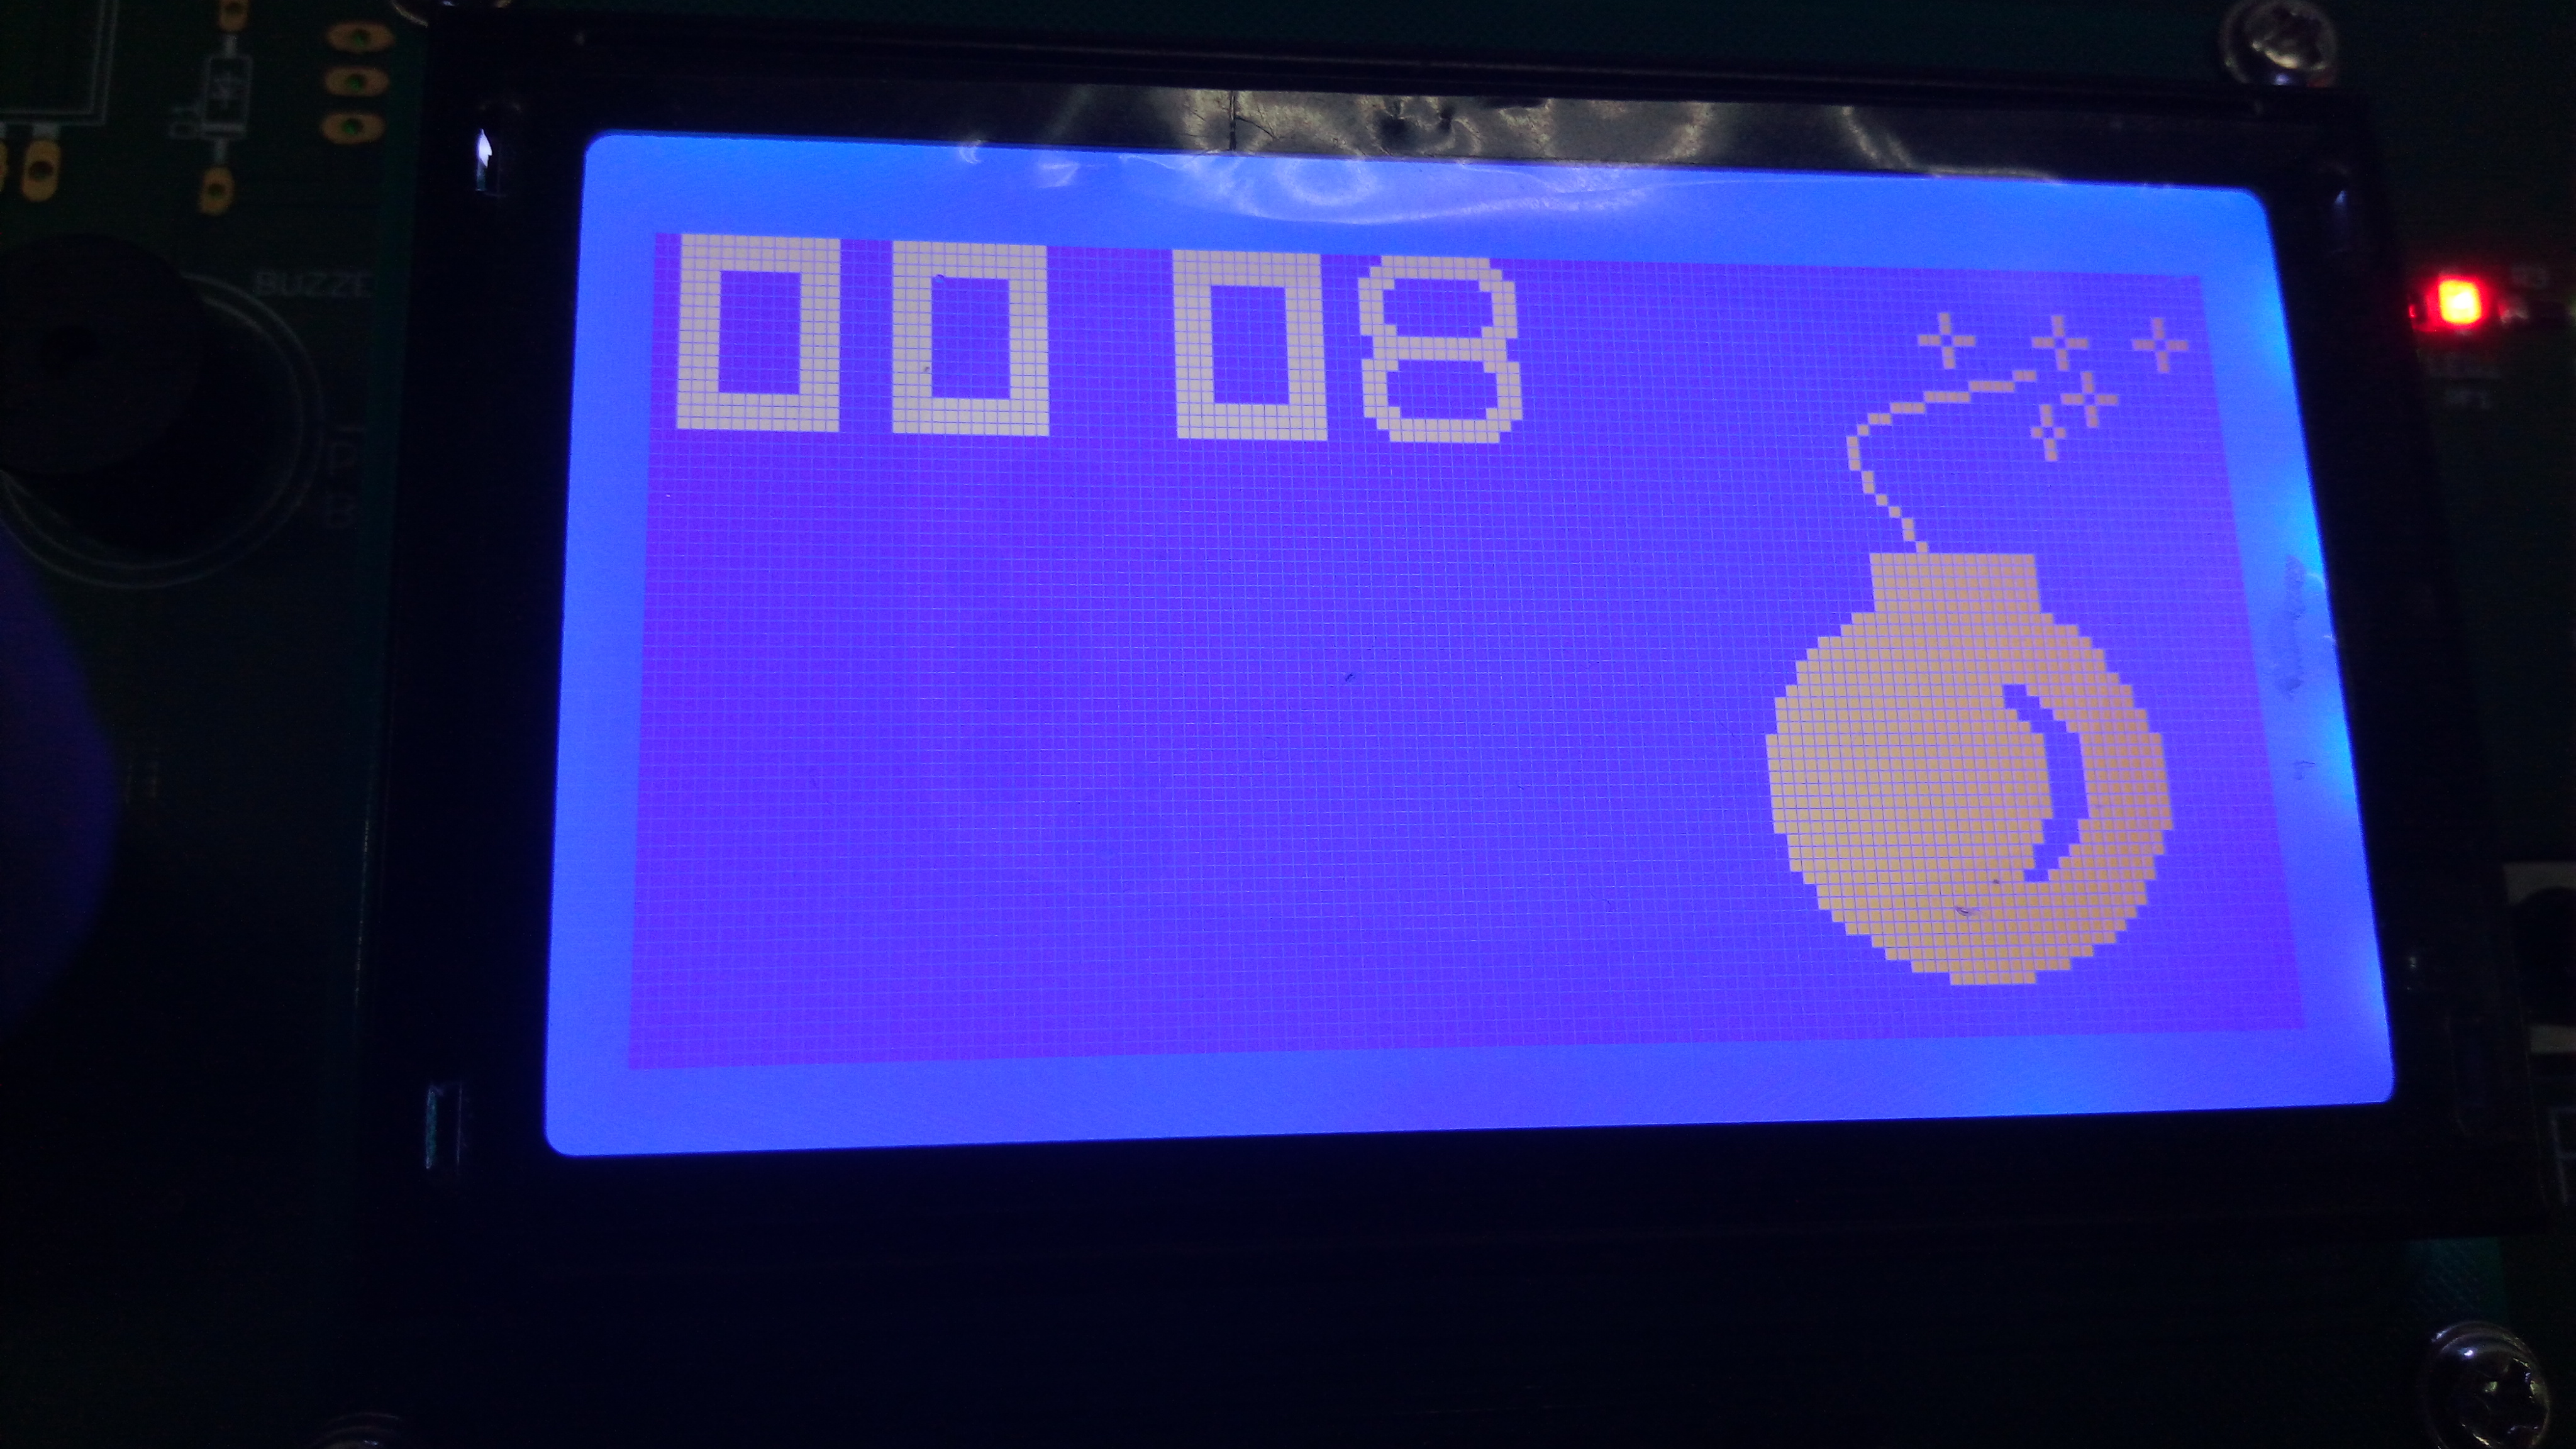
\includegraphics[width=8cm]{autoTimer2}
   \\Fig7: setTimer2
   \\[2\baselineskip]
 \end{center}
\section{bombExplode Mode:}
\begin{itemize}
    \item Once the timer value reaches zero then controller will enter in bombExplode mode.
    \item Create a bomb explosion animation which is displayed as shown in Fig8,Fig9 and Fig10. 
    \item After bomb animation is complete controller should go back in idle mode.
\end{itemize}
\begin{center}
   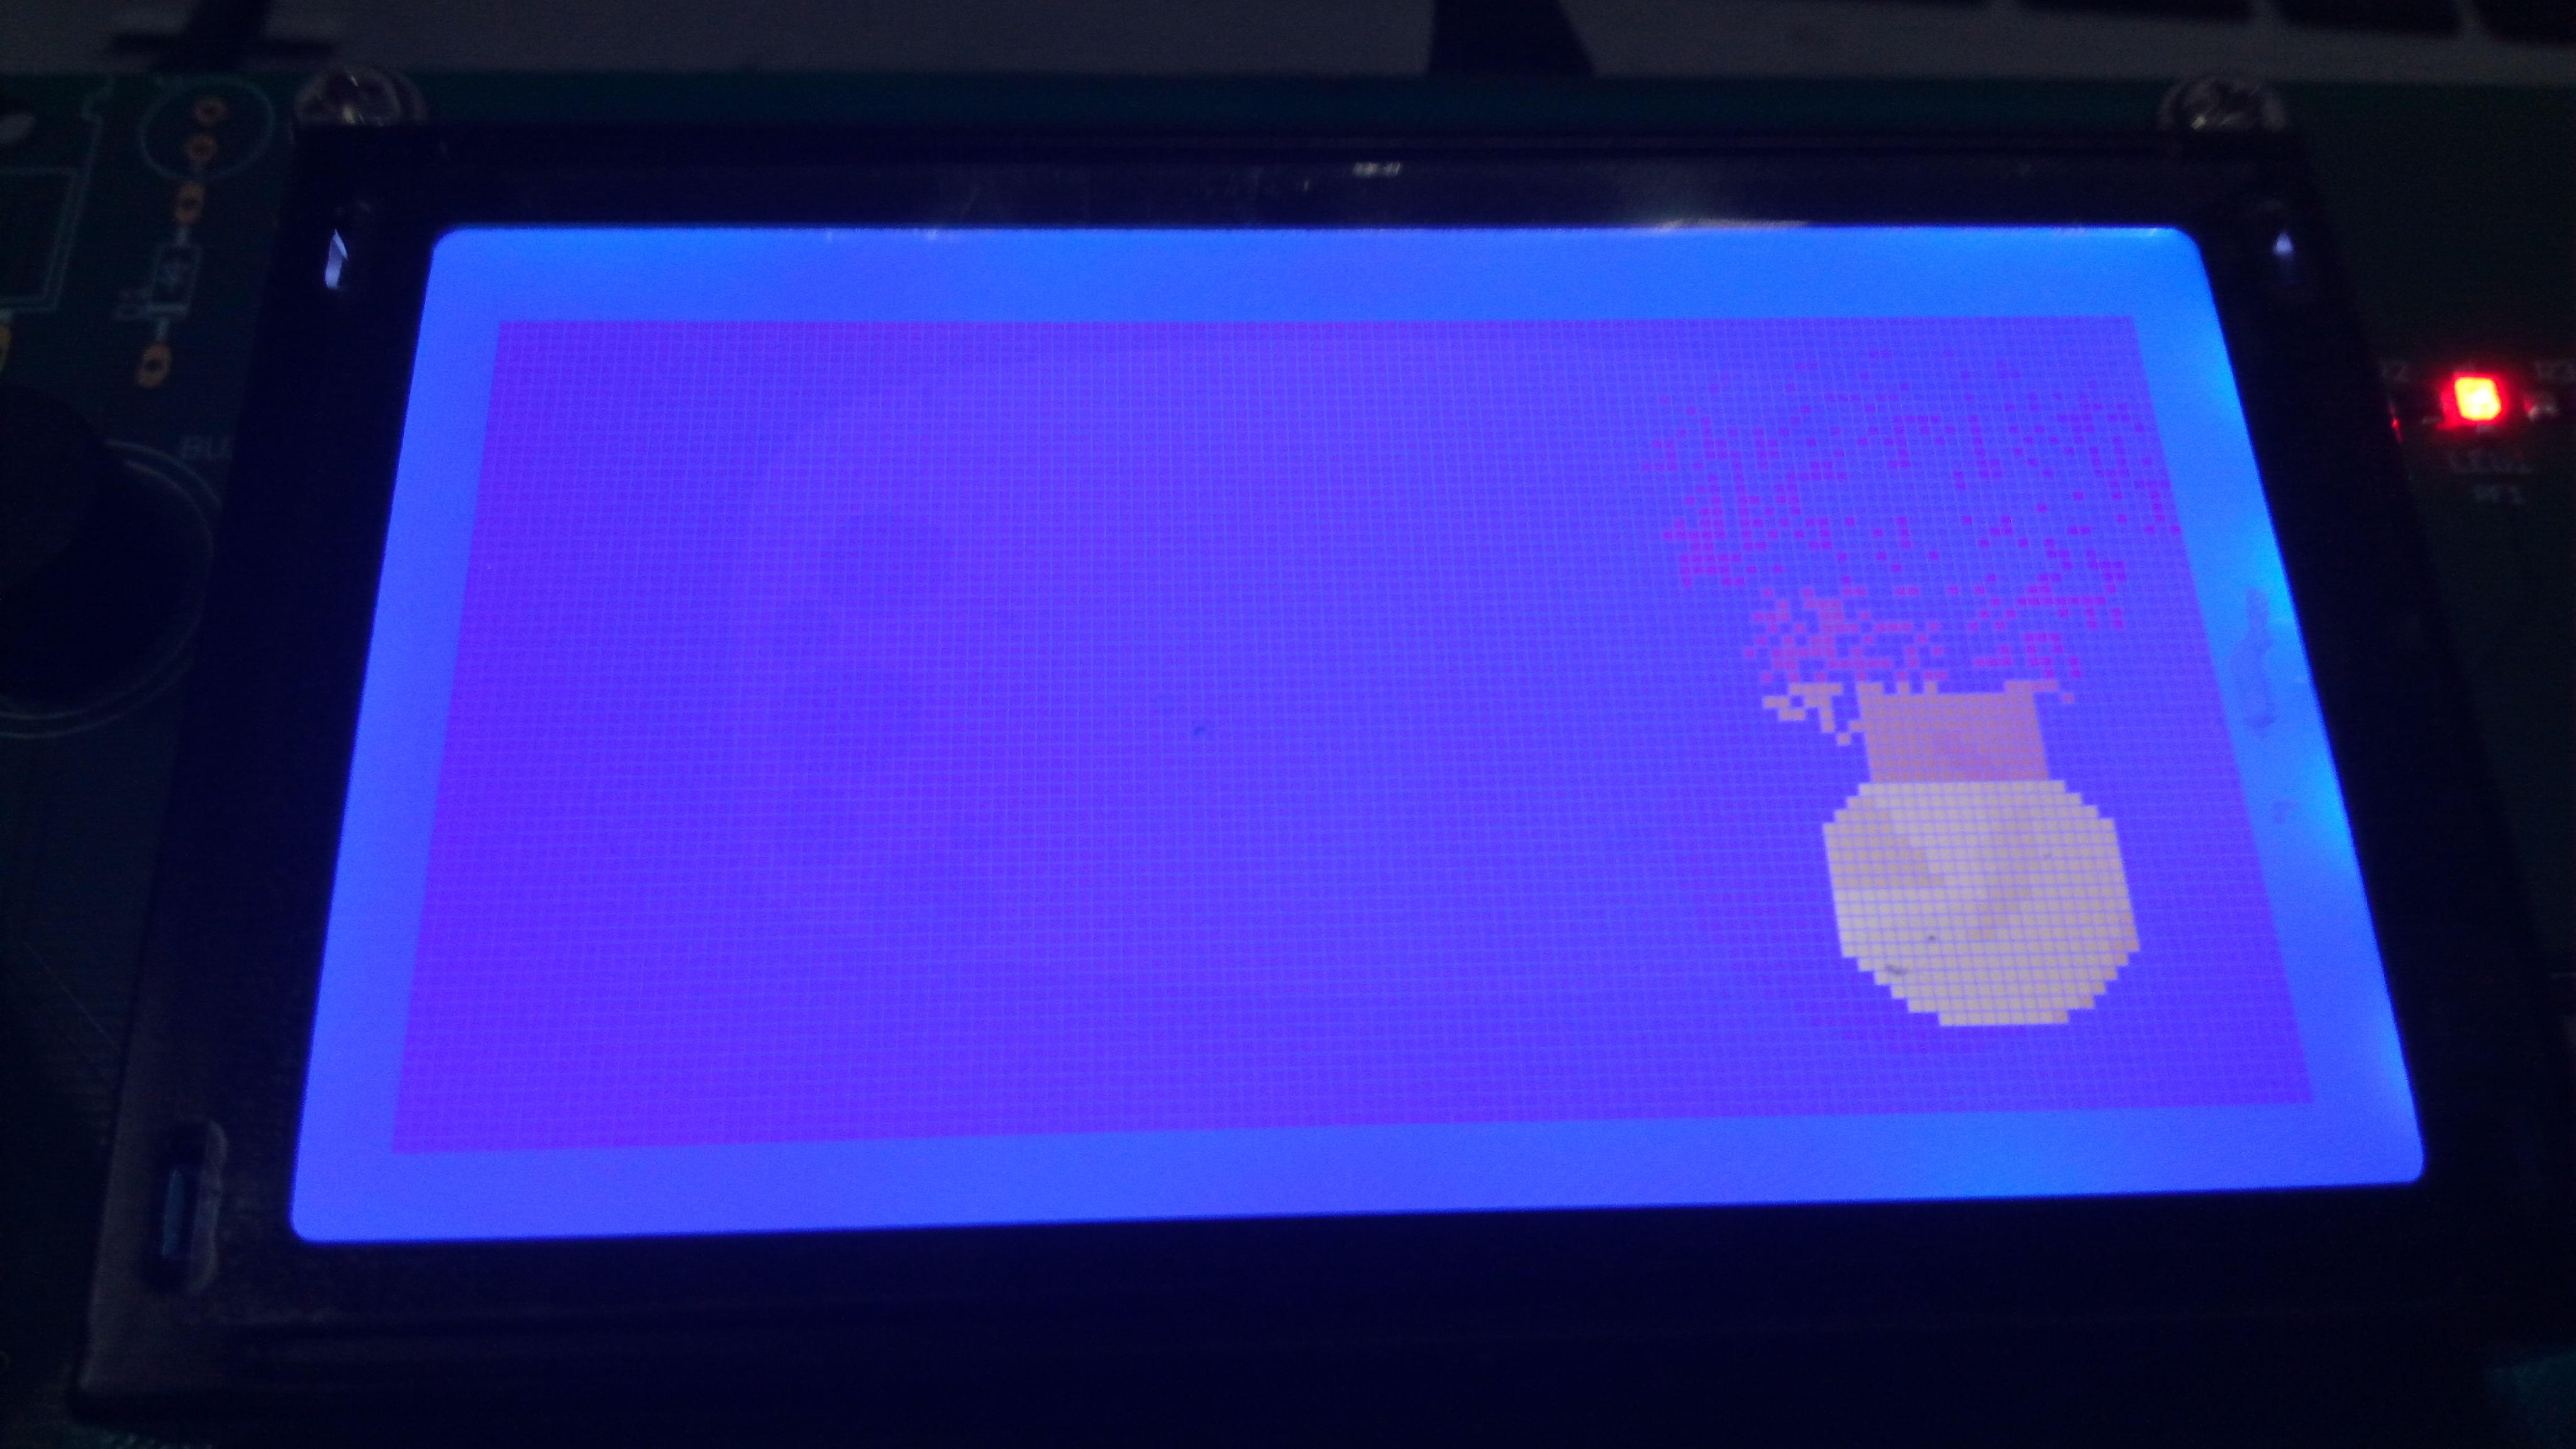
\includegraphics[width=8cm]{bombExplode1}
   \\Fig8: bombExplode1
   \\[2\baselineskip]
   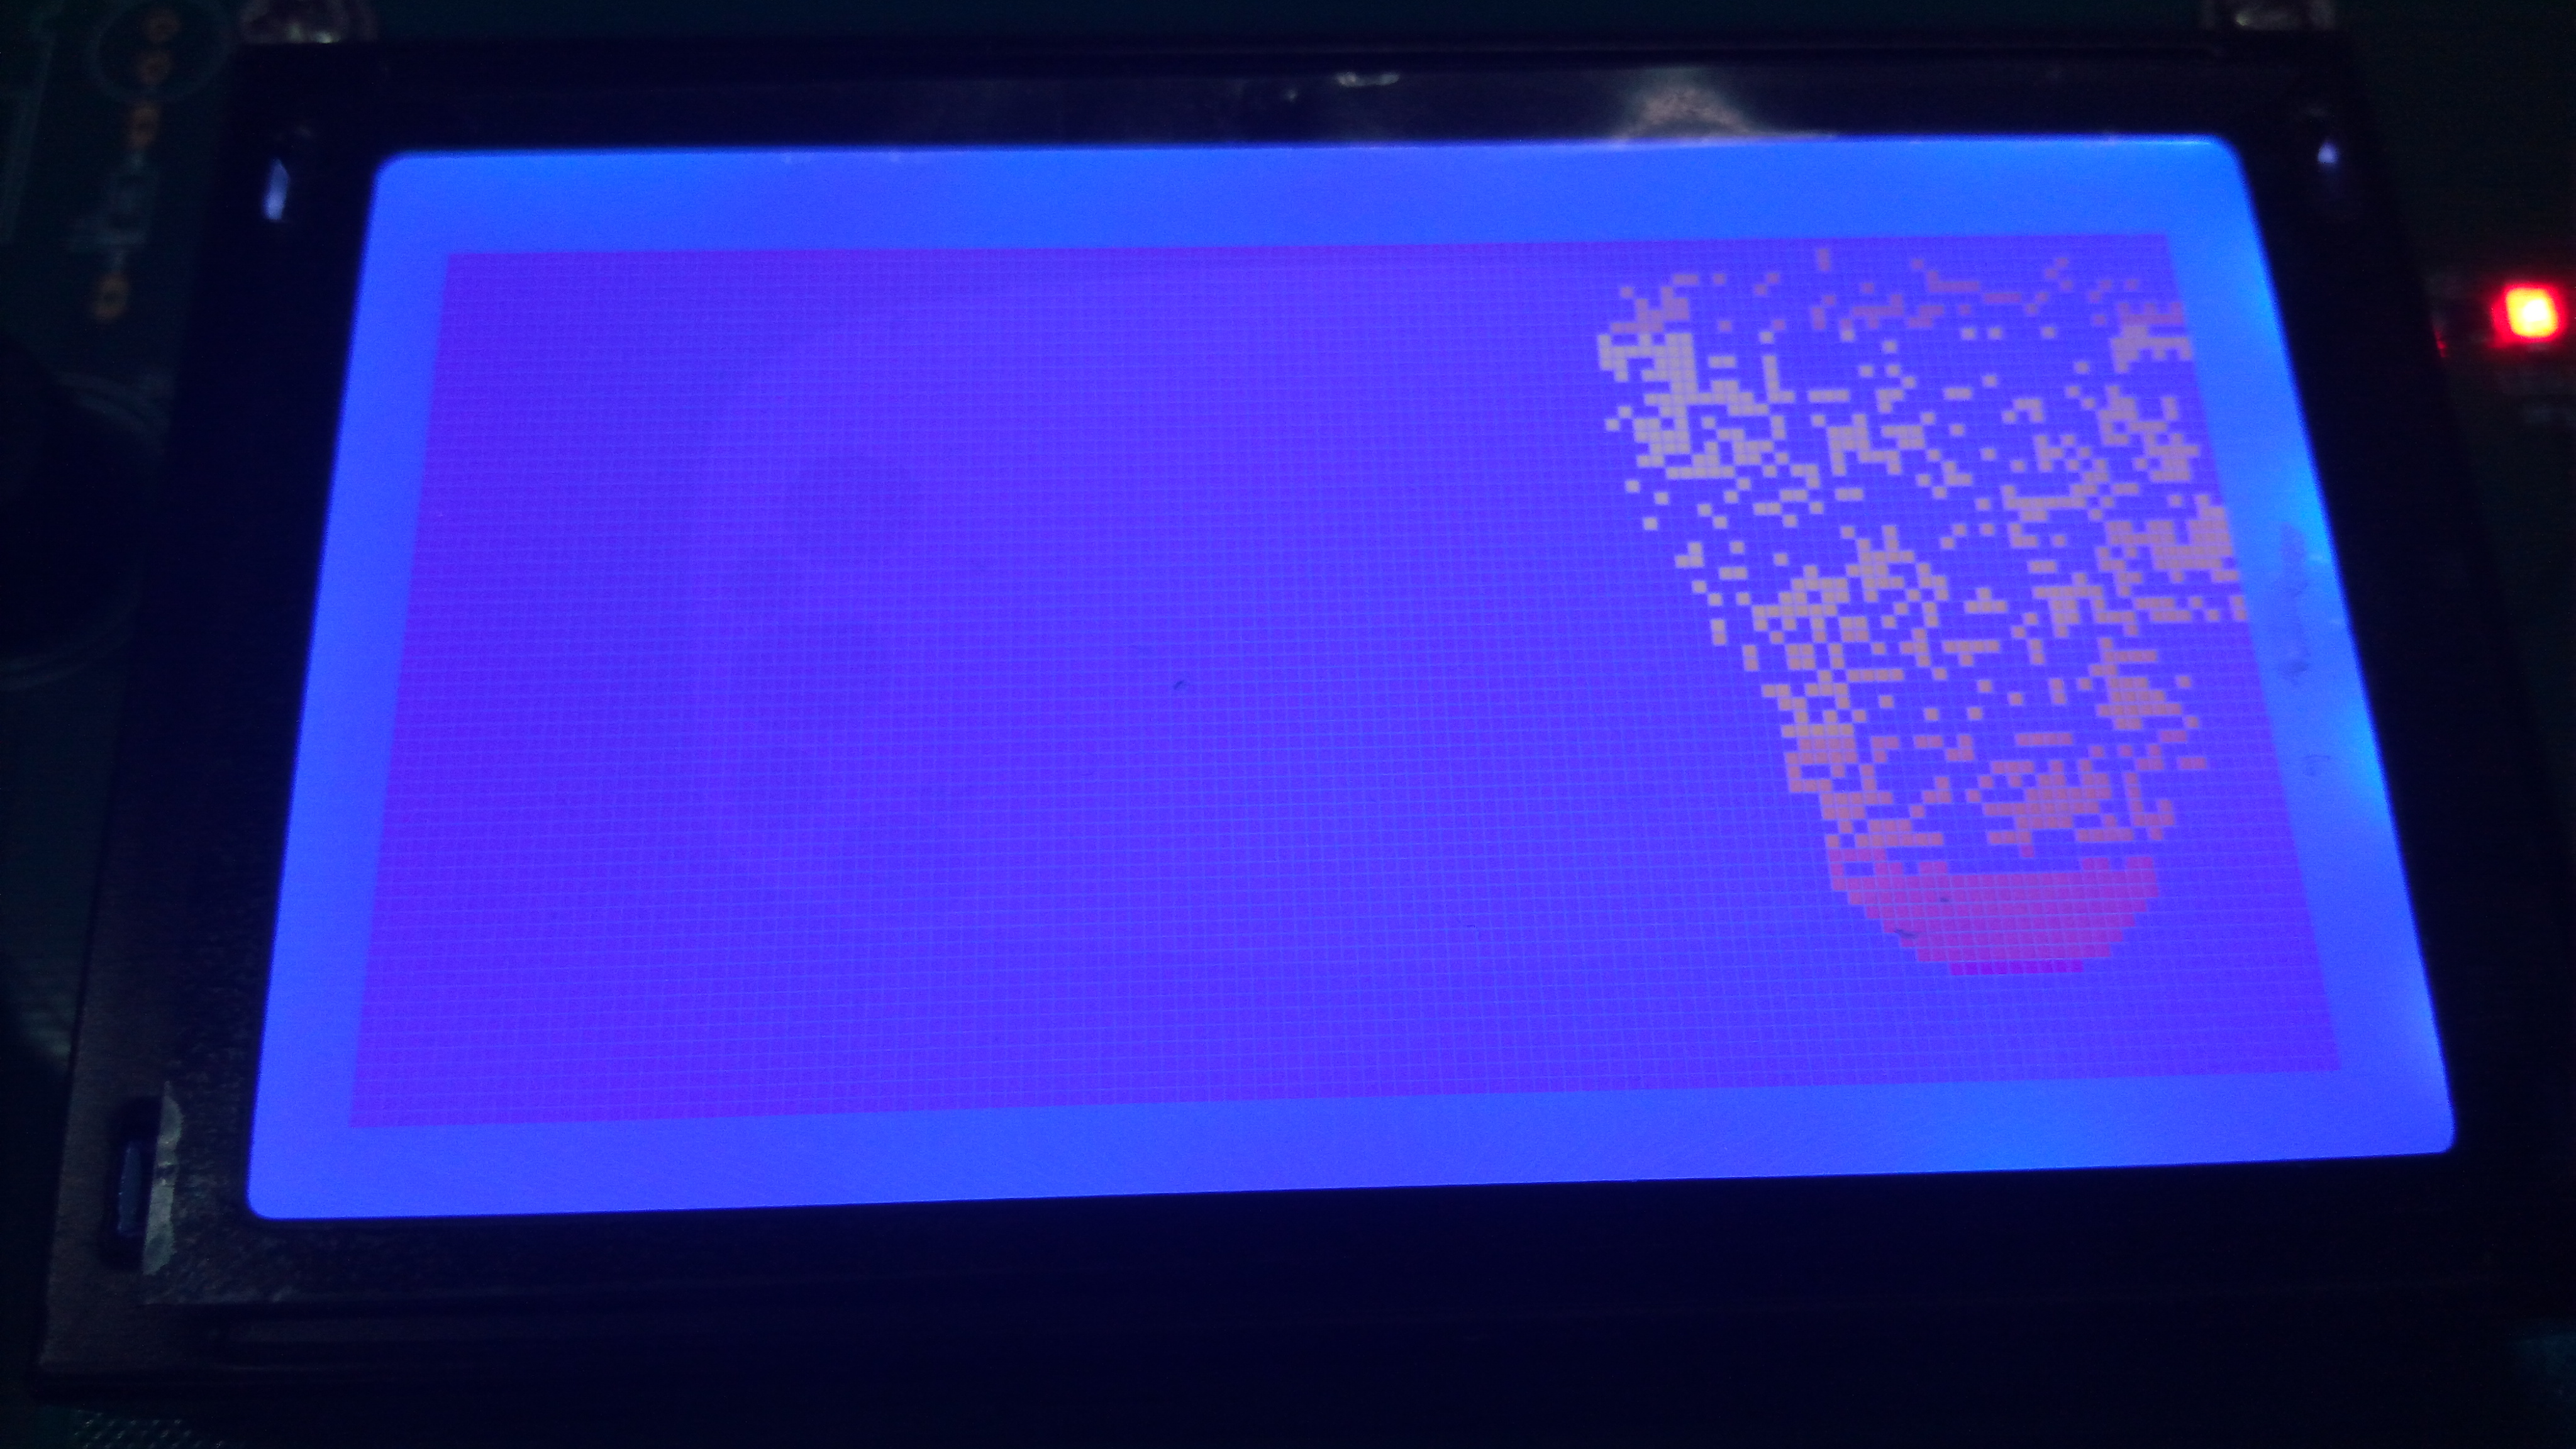
\includegraphics[width=8cm]{bombExplode2}
   \\Fig9: bombExplode2
   \\[2\baselineskip]
    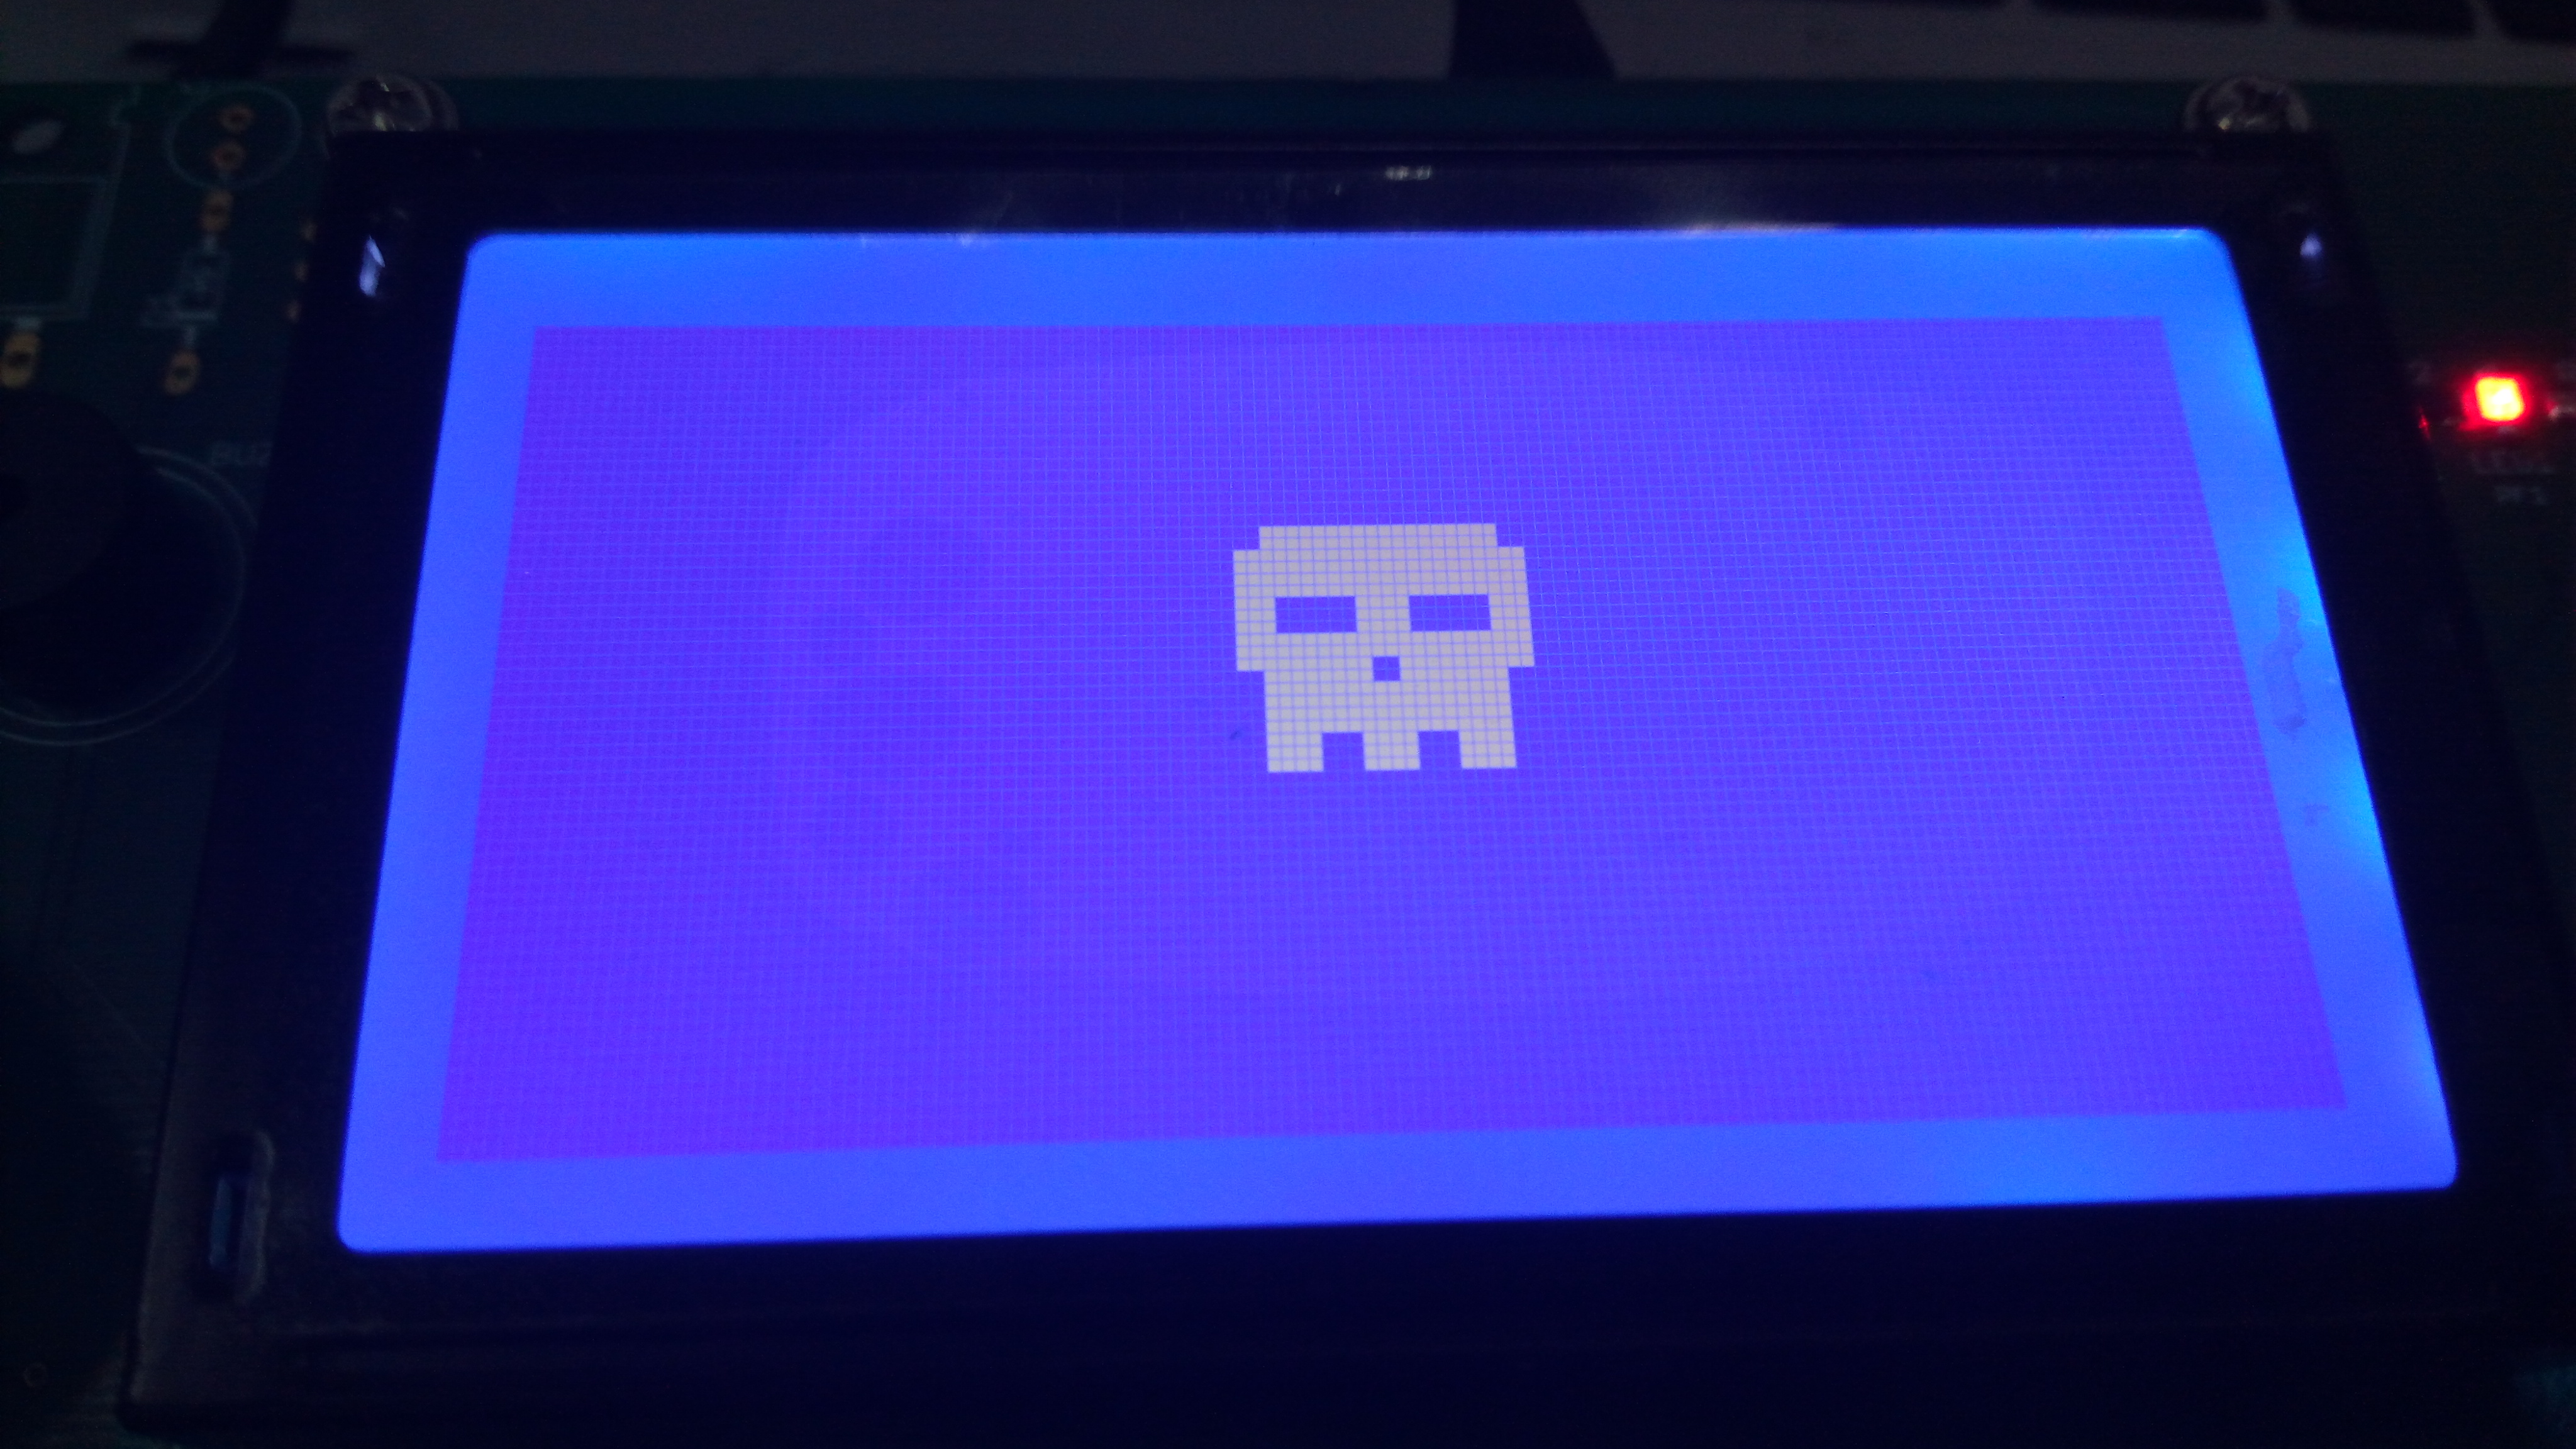
\includegraphics[width=8cm]{bombExplode3}
   \\Fig10: bombExplode3
   \\[2\baselineskip]
 \end{center}
\section{bombDiffused Mode:}
\begin{itemize}
    \item When controller is in autoTimer mode a password is kept to disarm the bomb.
    \item Password is a combination of switch press.
    \item Each switch can be pressed once. Password is 3 switch presses in a fixed sequence DOWN,UP,LEFT. sequence detector should be used.
    \item Upon correct entered password any small animation should be displayed as in Fig11.
    \item After animation is done the controller should enter back in idle mode.
\end{itemize}
\begin{center}
   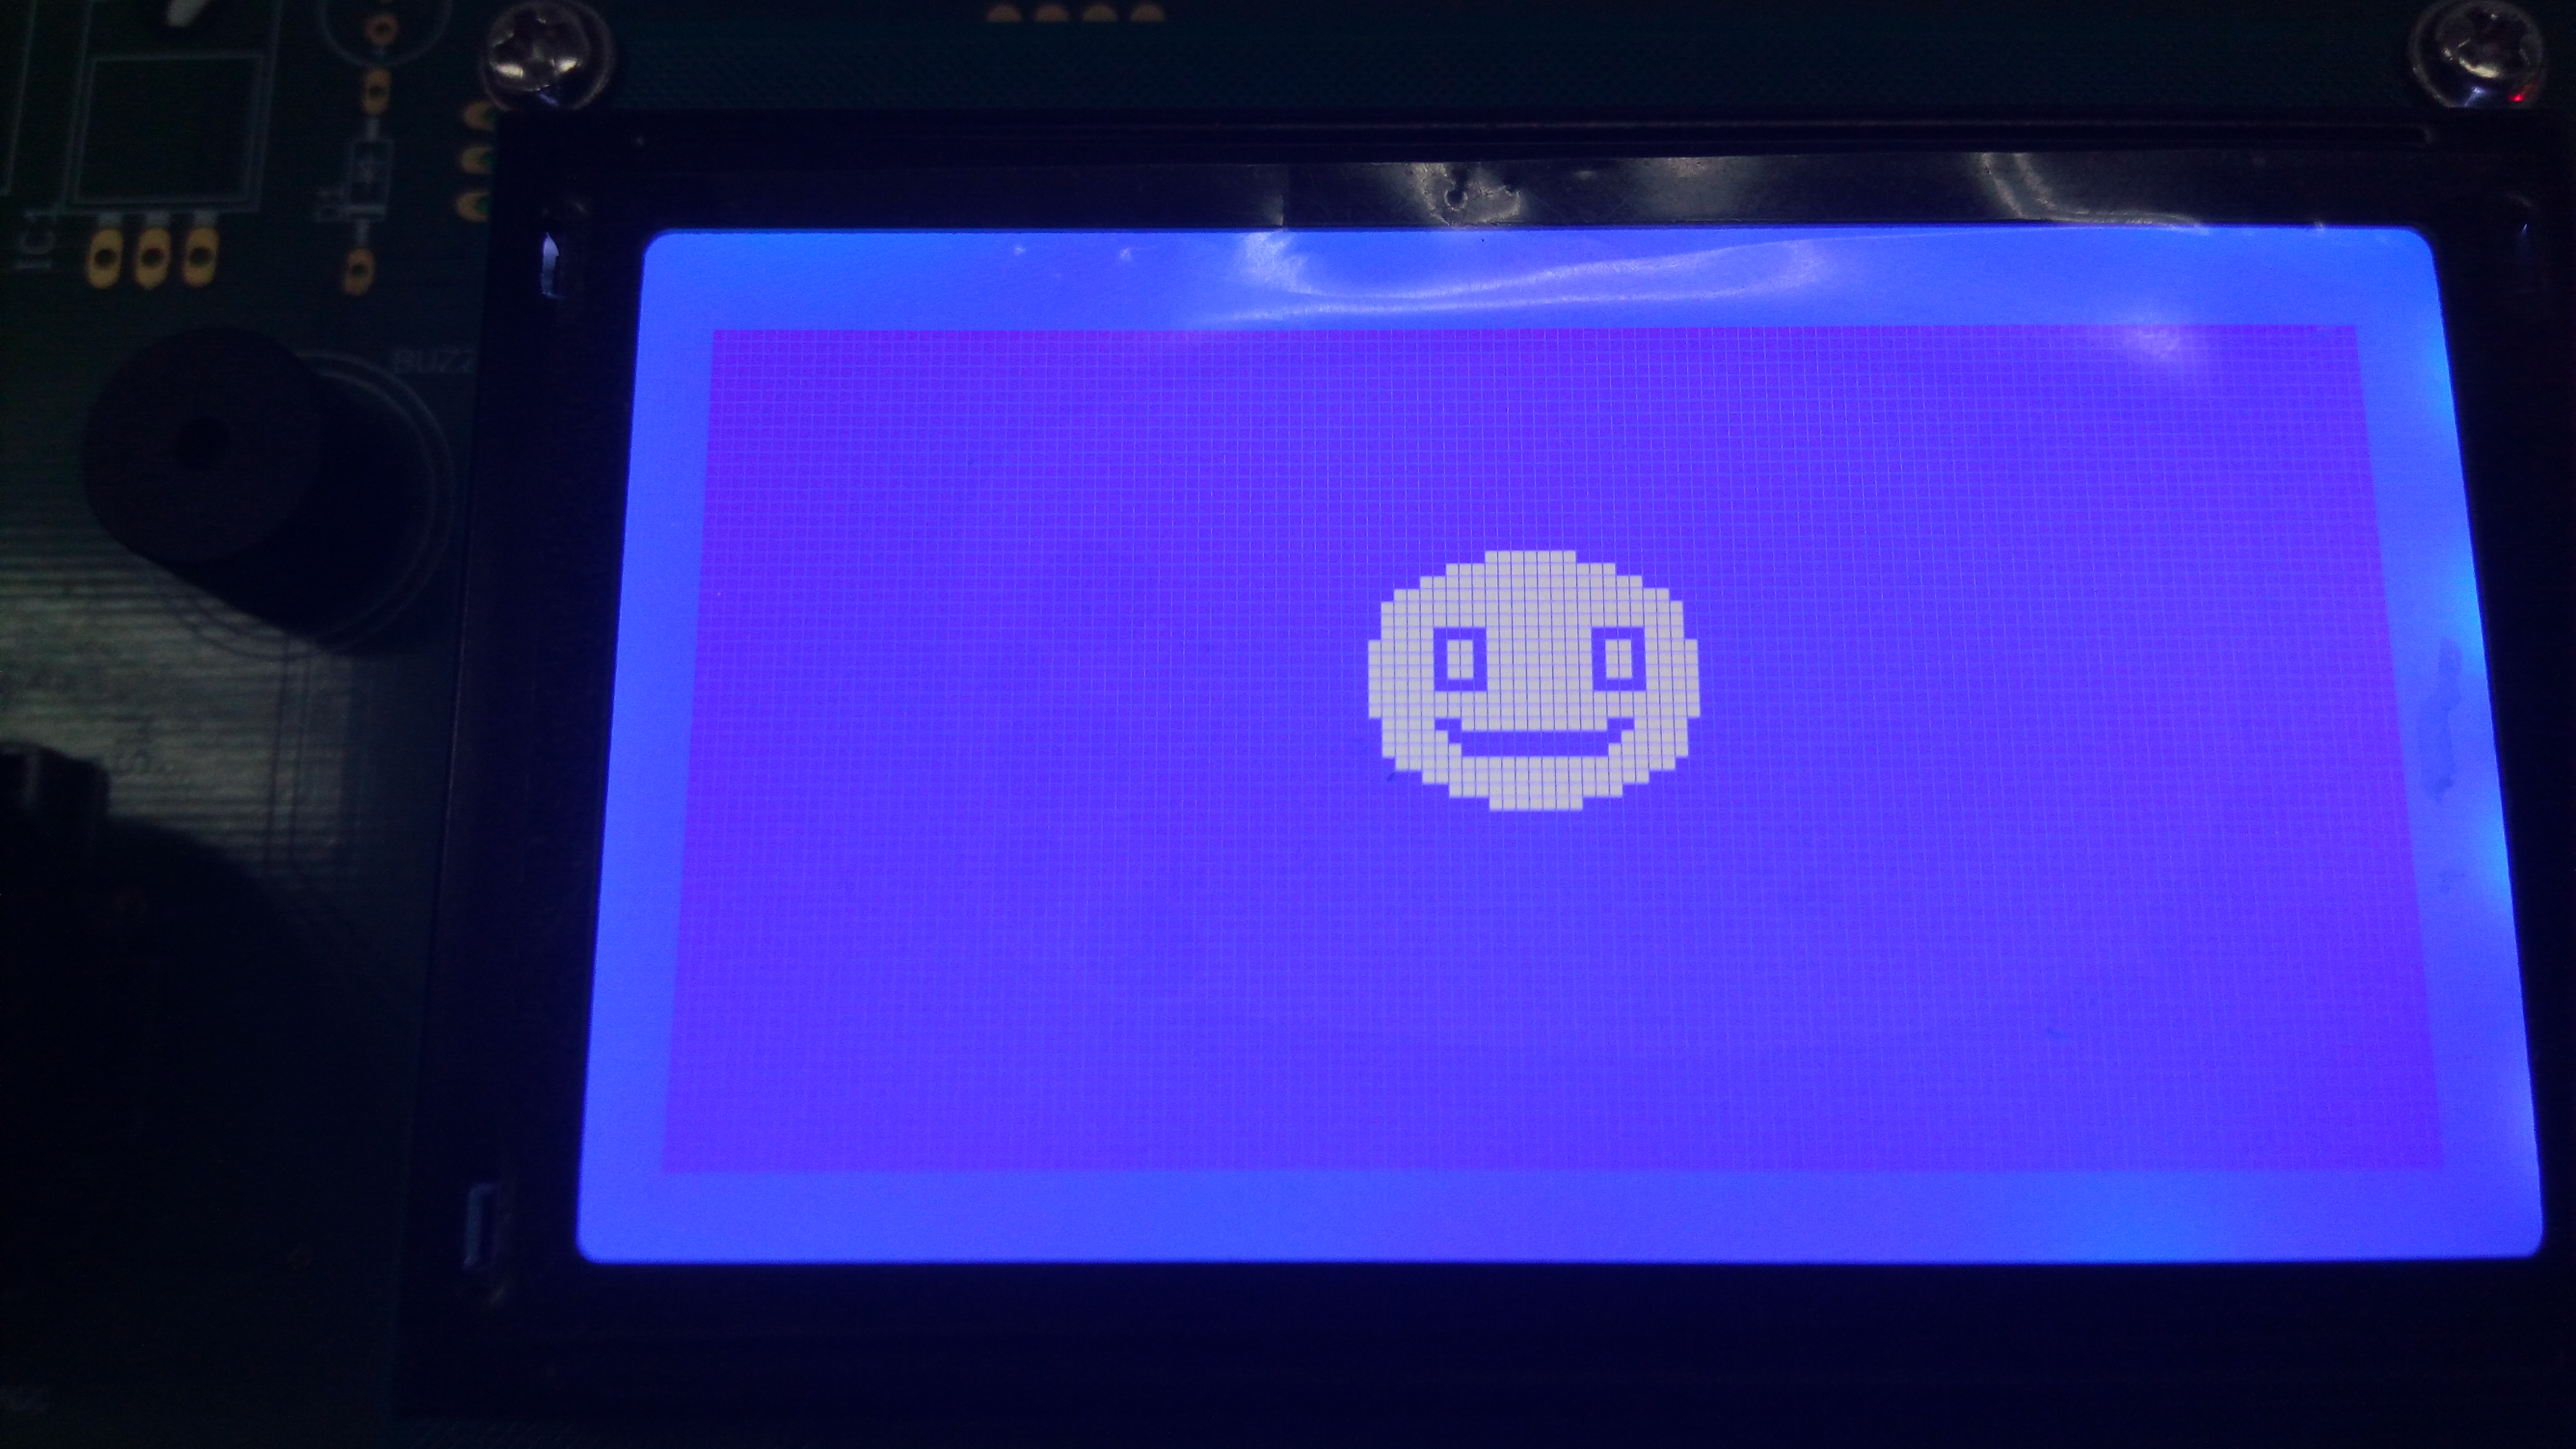
\includegraphics[width=8cm]{smiley}
   \\Fig11: smiley
   \\[2\baselineskip]
 \end{center}
\section{Demo and Submission:}
\begin{itemize}
    \item Draw the statechart for implementation of Timer Bomb.
    \item Show the output to TA and explain the working.
\end{itemize}
\begin{center}
\newline
   All The Best
  % \\[2\baselineskip]

 \end{center}
\end{document} 
